% arara: xelatex
% arara: xelatex
% arara: xelatex

% options:
% thesis=B bachelor's thesis
% thesis=M master's thesis
% czech thesis in Czech language
% english thesis in English language
% hidelinks remove colour boxes around hyperlinks

\documentclass[thesis=M,english]{FITthesis}[2018/05/30]

\usepackage{graphicx} %graphics files inclusion
% \usepackage{subfig} %subfigures
\usepackage{amsmath} %advanced maths
\usepackage{amssymb} %additional math symbols

\usepackage{dirtree} %directory tree visualisation

\usepackage[section]{placeins}
\usepackage{float}
\graphicspath{ {"C:/Users/Jakovcheski/Desktop/Stanford NER output/OneAnnotationAbstractBaseOnPageRank/"} }

% list of acronyms
% \usepackage[acronym,nonumberlist,toc,numberedsection=autolabel,nomain]{glossaries}
%\iflanguage{czech}{\renewcommand*{\acronymname}{Seznam pou{\v z}it{\' y}ch zkratek}}{}
% \makeglossaries

%\newcommand{\tg}{\mathop{\mathrm{tg}}} %cesky tangens
%\newcommand{\cotg}{\mathop{\mathrm{cotg}}} %cesky cotangens


\setcounter{tocdepth}{4} %define depth of showing in table of content
\setcounter{secnumdepth}{4} %define depth of showing in table of content


% % % % % % % % % % % % % % % % % % % % % % % % % % % % % % % % % % % 
% % % % % % % % % % % % % % % % % % % % % % % % % % % % % % % % % % % 
\department{Department of software engineering}
\title{Domain-specific Name Entity Recognition}
\authorGN{Bogoljub} %author's given name/names
\authorFN{Jakovcheski} %author's surname
\authorWithDegrees{Bc. Bogoljub Jakovcheski} %author's name with academic degrees
\author{Bogoljub Jakovcheski} %author's name without academic degrees
\supervisor{Ing. Milan Dojchinovski, Ph.D.}
\acknowledgements{I would like to thank my family and friends for support during writing this thesis.}
\abstractCS{}
\abstractEN{}
\placeForDeclarationOfAuthenticity{Prague} %where you have signed the declaration
\keywordsCS{}
\keywordsEN{}
\declarationOfAuthenticityOption{4} %select as appropriate, according to the desired license

\begin{document}
% \newacronym{LZW}{LZW}{Lempel Ziv Welch}
% \newacronym{RLE}{RLE}{Run-Length Encoding}

\begin{introduction}

\section{Motivation}
	Nowadays Named Entity Recognition (NER) is far away from perfectly matching entities in text. State-of-the-art NER systems for English produce near-human performance. For example, the best system entering MUC-7 scored 93.39\% of F-measure while human annotators scored 97.60\% and 96.95\%. %[https://en.wikipedia.org/wiki/Named-entity_recognition]
	  
\section{Goals of the thesis}	
	%The main goal of the thesis is to show (test) does extracting information from a global domain gives us better results that extracting information from a specific domain, for example politics domain or any other domain.
	
	The main goal of the thesis is to create a domain specific models and try to get closer, or event better F1-score to the human F1-score. Then creating a smaller and larger models and their impact of scoring based on main model. And finally creating a coarse grained and fine grained models and monitoring their F1-score.   
	
\section{Thesis outline}
	

\end{introduction}

\chapter{Background and related work}\label{}

	%This thesis was submitted at Czech Technical University in Prague (see Figure~\ref{fig:logo}).
	
	%\begin{figure}[H]\centering
		%\includegraphics{cvut-logo-bw}
		%\caption{CTU logo}\label{fig:logo}
	%\end{figure}

\section{Information extraction}

	Information extraction first appears in late 1970s within NLP field. %[https://www.slideshare.net/rubenizquierdobevia/information-extraction-45392844] 	 
Based on Wikipedia\cite{Wikipedia}, Information extraction (IE) is the task of automatically extracting structured information from unstructured and/or semi-structured machine-readable documents. In most of the cases this activity concerns processing human language texts by means of natural language processing (NLP). Recent activities in multimedia document processing like automatic annotation and content extraction out of images/audio/video could be seen as information extraction. [https://en.wikipedia.org/wiki/Information\_extraction] \cite{wiki:IE}
\linebreak Another view of that what Information extraction is that automatically building a relational database from information contained in unstructured text. Unlike linear-chain models, general CRFs can capture long distance dependencies between labels. [http://people.cs.umass.edu/~mccallum/papers/crf-tutorial.pdf]
\linebreak To understand better what IE is we can use example in [https://ontotext.com/knowledgehub/fundamentals/information-extraction/], extracting information for mail message and adding to your Calendar. Millions of people use this on their daily basis and they are not aware of that how that works and what technology is used for that.
\linebreak Figure~\ref{fig:InformationExtraction} gives us closer look of what Information extraction (IE) is, and how State-of-the-Art algorithms transforms unstructured text to structured sequences understandable for machines. 

	\begin{figure}[H]\centering
		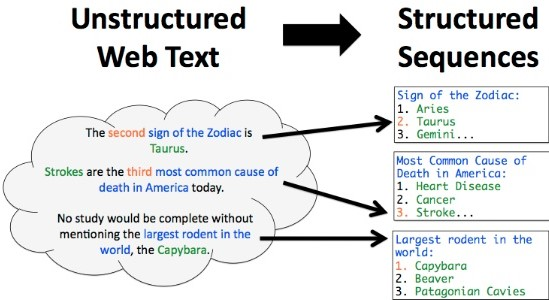
\includegraphics[width=\textwidth]{information-extraction}
		\caption{Information extraction, downloaded from https://www.slideshare.net/rubenizquierdobevia/information-extraction-45392844}\label{fig:InformationExtraction}
	\end{figure}
%http://people.cs.umass.edu/~mccallum/papers/crf-tutorial.pdf
%https://web.stanford.edu/~jurafsky/slp3/21.pdf
%https://en.wikipedia.org/wiki/Information_extraction
%https://ontotext.com/knowledgehub/fundamentals/information-extraction/

\section{Named Entity Recognition}
Named Entity Recognition (NER) is the problem of identifying and classifying proper names in text, including locations, such as China; people, such as George Bush; and organizations, such as the United Nations. The named-entity recognition task is, given a sentence, first to segment which words are part of entities, and then to classify each entity by type (person, organization, location, and so on). The challenge of this problem is that many named entities are too rare to appear even in a large training set, and therefore the system must identify them based only on context.
\linebreak One approach to NER is to classify each word independently as one of either Person, Location, Organization, or Other (meaning not an entity). The problem with this approach is that it assumes that given the input, all of the named entity labels are independent. In fact, the named-entity labels of neighboring words are dependent; for example, while New York is a location, New York Times is an organization. [http://people.cs.umass.edu/~mccallum/papers/crf-tutorial.pdf section 1.2.2.2]

%The first step in most IE tasks is to find the proper names or named entities mentioned in a text. The task of named entity recognition (NER) is to find each mention of a named entity in the text and label its type. What constitutes a named entity type is application specific; these commonly include people, places, and organizations but also more specific entities from the names of genes and proteins(Cohen and Demner-Fushman, 2014) to the names of college courses (McCallum,2005).%[https://web.stanford.edu/~jurafsky/slp3/21.pdf]

Named-entity recognition (NER) (also known as entity identification, entity chunking and entity extraction) is a subtask of information extraction (IE) that seeks to locate and classify named entities in text into pre-defined categories such as the names of persons, organizations, locations, expressions of times, quantities, monetary values, percentages, etc.

Most research on NER systems has been structured as taking an unannotated block of text, such as this one:

Jim bought 300 shares of Acme Corp. in 2006.

And producing an annotated block of text that highlights the names of entities:

[Jim]Person bought 300 shares of [Acme Corp.]Organization in [2006]Time.

In this example, a person name consisting of one token, a two-token company name and a temporal expression have been detected and classified.
[https://en.wikipedia.org/wiki/Named-entity\_recognition]
\linebreak Figure~\ref{fig:StanfordNER} shows how one NER application can look like. The text in example is predefined in Stanford NER application and loaded model (Classifier) is also trained by Stanford [https://nlp.stanford.edu/software/CRF-NER.html\#Models].

	\begin{figure}[H]\centering
		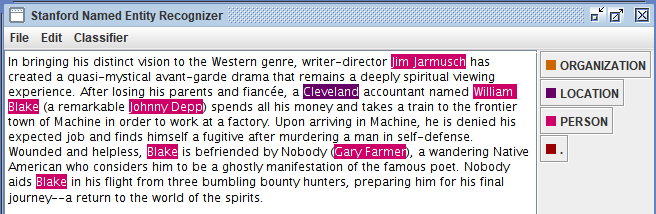
\includegraphics[width=\textwidth]{NER-Stanford}
		\caption{Stanford NER GUI with 3 classes model (Location, Person, Organization)}\label{fig:StanfordNER}
	\end{figure}
	
\subsection{$F_{1}$ score}
The success of NER systems is exposed to $F_{1}$ score (F-score or F-measure). $F_{1}$ score  is a measure of a test's accuracy. It considers both the precision p  and the recall r of the test to compute the score: p is the number of correct positive results divided by the number of all positive results returned by the classifier, and r is the number of correct positive results divided by the number of all relevant samples (all samples that should have been identified as positive). The F1 score is the harmonic average of the precision and recall, where an F1 score reaches its best value at 1 (perfect precision and recall) and worst at 0. 
Written in formula, the $F_{1} =2\cdot \frac{precision \cdot recall}{precision + recall}$ [https://en.wikipedia.org/wiki/F1\_score]


\subsection{Stanford NER}\label{Stanford NER}
Stanford NER is a Java implementation of a Named Entity Recognizer. Named Entity Recognition (NER) labels sequences of words in a text which are the names of things, such as person and company names, or gene and protein names. It comes with well-engineered feature extractors for Named Entity Recognition, and many options for defining feature extractors. Included with the download are good named entity recognizers for English, particularly for the 3 classes (PERSON, ORGANIZATION, LOCATION), and we also make available on this page various other models for different languages and circumstances, including models trained on just the CoNLL 2003 English training data.

Stanford NER is also known as CRFClassifier. The software provides a general implementation of (arbitrary order) linear chain Conditional Random Field (CRF) sequence models. That is, by training your own models on labeled data, you can actually use this code to build sequence models for NER or any other task.[https://nlp.stanford.edu/software/CRF-NER.html]

\section{RDF/NIF}
The Resource Description Framework (RDF) is a family of World Wide Web Consortium (W3C) specifications originally designed as a metadata data model. It has come to be used as a general method for conceptual description or modeling of information that is implemented in web resources, using a variety of syntax notations and data serialization formats. It is also used in knowledge management applications. [https://en.wikipedia.org/wiki/Resource\_Description\_Framework]
\linebreak More precisely RDF is a standard model for data interchange on the Web. RDF has features that facilitate data merging even if the underlying schemas differ, and it specifically supports the evolution of schemas over time without requiring all the data consumers to be changed. [https://www.w3.org/RDF/]
\linebreak Natural Language Processing Interchange Format (NIF) is an RDF-based format. The classes to represent linguistic data are defined in the NIF Core Ontology. All ontology classes are derived from the main class nif:String which respresents strings of Unicode characters.[https://www.w3.org/2015/09/bpmlod-reports/nif-based-nlp-webservices/\#natural-language-\%processing-interchange-format-nif] [http://aksw.org/Projects/NIF.html]. 
%http://wiki.dbpedia.org/dbpedia-nif-dataset
%http://persistence.uni-leipzig.org/nlp2rdf/ontologies/nif-core/nif-core.html
%https://www.w3.org/2015/09/bpmlod-reports/nif-based-nlp-webservices/#natural-language-%processing-interchange-format-nif
%http://lov.okfn.org/dataset/lov/vocabs/nif
%http://aksw.org/Projects/NIF.html

\section{Domain specific Named Entity Recognition}
Traditionally Named Entity Recognition (NER) systems have been built using available annotated datasets (like CoNLL, MUC) and demonstrate excellent performance. However, these models fail to generalize onto other domains like Sports and Finance where conventions and language use can differ significantly. Furthermore, several domains do not have large amounts of annotated labeled data for training robust Named Entity Recognition models. [https://arxiv.org/pdf/1612.00148.pdf]
With specifying the domain we can create a bigger model with more annotated words and reading the whole text will be same or even faster that reading text with a global domain.  
%https://arxiv.org/pdf/1612.00148.pdf

\section{DBpedia ontology}
%http://wiki.dbpedia.org/services-resources/ontology
%http://mappings.dbpedia.org/server/ontology/classes
The DBpedia Ontology is a shallow, cross-domain ontology, which has been manually created based on the most commonly used infoboxes within Wikipedia. The ontology currently covers 685 classes which form a subsumption hierarchy and are described by 2,795 different properties.

Since the DBpedia 3.7 release, the ontology is a directed-acyclic graph, not a tree. Classes may have multiple superclasses, which was important for the mappings to schema.org. A taxonomy can still be constructed by ignoring all superclasses except the one that is specified first in the list and is considered the most important. [http://wiki.dbpedia.org/services-resources/ontology]

Dbpedia ontology classes can be found here [http://mappings.dbpedia.org/server/ontology/classes/]

The DBpedia Ontology currently contains about 4,233,000 instances. Figure~\ref{fig:Dbpedia-ontology} shows the number of instances for several classes within the ontology. [http://wiki.dbpedia.org/services-resources/ontology]

	\begin{figure}[H]\centering
		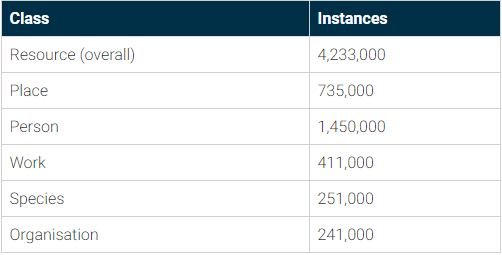
\includegraphics[width=\textwidth]{Dbpedia-ontology}
		\caption{Dbpedia Ontology - Instances per class}\label{fig:Dbpedia-ontology}
	\end{figure}

\section{Evaluation/training datasets}
For the aim of our experiments we have trained 57 datasets. For training we've used Stanford NER application explained in subsection~\ref{Stanford NER}. We have two types of datasets, coarse-grained and fine-grained, also those types are divided in to specific domains and a global domain. To give an illustration, for model with 100 retrieved abstract we will have 4 coarse-grained models (global domain and 3 specific domains), and similarly for a fine-grained models.




%%%%%%%%%%%%%%%%%%%%%%%%%%%%%NEW CHAPTER%%%%%%%%%%%%%%%%%%%%%%%%%%%%%%%%%%%%%%%%%%%%%%%%%%%
\chapter{Domain specific named entity recognition}\label{}

There are parameters of the computer used for tests shown in Table \ref{tab:PCparam}.
\begin{table}[H]\centering
	\caption{Testing computer parameters}
	\label{tab:PCparam}
	\begin{tabular}{|l|r|}
	\hline \multicolumn{1}{|c|}{\textbf{Part}} & \multicolumn{1}{|c|}{\textbf{Description}} \\\hline
	CPU & 2.00 GHz Intel(R) Core(TM) i5-4310U \\
	MEM & 16 GB DDR3L\\
	OS & x86\_64 Windows 10 Pro\\
	DISK & 240GB SSD Kingston\\\hline
	\end{tabular}
\end{table}

\section{Data pre-processing}
First of all we downloaded 2 datasets from Dbpedia NIF Datasets [http://wiki.dbpedia.org/dbpedia-nif-dataset] for English language in .ttl format. Those datasets are: 
\begin{itemize}
	\item nif-context (or nif-abstract-context): the full text of a page as context (including begin and end index)
	\item nif-text-links: all in-text links to other DBpedia resources as well as external references
\end{itemize}  
Another dataset that we needed was Dbpedia instance types dataset, downloaded from here [http://wiki.dbpedia.org/downloads-2016-04] also in .ttl format. This dataset contains all types from nif-text-links that occurrence at nif-abstract-context.
So how all this dataset are connected between themselves? Let say that we have abstract for Alexander the Great. In nif-text-links file we have all words from abstract that has annotation, but we still don't know their type. So here comes instance types file where based on link from nif-text-link (eg.http://dbpedia.org/resource/Philip\_II\_of\_Macedon) we can find the type of annotated word (word Philip II has ontology type Monarch), but of coarse there can be a case that some words cannot be found on instance types file and automaticly have no type, or in our case ontology type O (O like Other).
But know, let us explain deeply how we process and clean data from dataset. First we define small test dataset to check how fast we can process data. Running that dataset on downloaded files without any cleaning on data takes too long. So we said that converting the datasets from .ttl to .hdt (binary format) with rdf/hdt tool [http://www.rdfhdt.org/] will be faster. So we converted the datasets and reruned the algorithm again. There were some improvements, but not satisfying for our purposes. Our next solution was to clean datasets from unused data for our aims. The final result after cleaning the datasets was a smaller datasets, for instance nif-abstract-context file from 7.78GB now has 2.99GB, another big improvement was nif-text-links file who is reduced to 10.5GB from 44.6GB and at the end we also clean instance types file, but here we don't record any mayor memory improvements. Again we rerun the algorithm, of course there were improvements, but as well as previous the time that algorithm runs, was not acceptable for us. To give an illustration the time needed to find all types from one abstract in worst case, to read nif-text-links and instance type files until end was around 3.5 minutes. Therefore once more we converted our cleaned datasets from RDF format to binary format. And how in previous running there were again improvements, but those improvements doesn't fulfill our expectations. The final think that we have to save us was creating a dataset tree. For nif-text-links file we created a tree where we have folders from "a-z", also special characters folders and other folder(this folder contains data that have a lower occurrence, let say \& character or letters that are not part of English alphabet), folders from "a-z" has subfolders also from a-z. 
\linebreak To give a closer look how we create that tree, let say that we have an abstract for Volkswagen Golf MK3, so the link for that abstract would be http://dbpedia.org/resource/Volkswagen\_Golf\_Mk3 and this link will be stored to "v" folder and "o" subfolder. With this we have a smaller dataset where we can read whole one very fast.

For instance types file we modified the algorithm for creating a data tree. Here because of lower range data we have created only files from "a-z" and of coarse special characters
Finally we rerun the algorithm, and the time to process one abstract at worst case takes no more that 1 minute. Now we were ready to take next steps to retrieve types (subsection~\ref{typesRetrieval}) and create domains (subsection~\ref{domainSpecification}) and prepare data for Stanford NER (subsection~\ref{StanfordNERoutput}).             


\section{Types retrieval}\label{typesRetrieval}
After we solved the problem of that how effectively run the algorithm to find all types from the abstract, next issue was which types we want to be part of our domains and also which types we want to retrieve from Dbpedia. Worth mentioning that we will use the same ontology types for retrieving the abstracts links from Dbpedia and creating a domain models. For example the type "Politician" will be used to retrieve links from Dbpedia that has that type, and also "Politician" type will be use to annotated words, for instance Barack Obama will have type of "Politician" (we will give more details on subsection~\ref{StanfordNERoutput}).

In Dbpedia ontology classes page [http://mappings.dbpedia.org/server/ontology/classes/] we can see all types that Dbpedia has. Those ontology types are the same in instance types file also. Now we are facing with the fact that if we choose very small group of ontology types, at the experiment point we will have minor range of annotated words and experiments won't be relevant. On the other hand, if we go too deep to ontology types, we will have a lot of annotated words, but training the model take a lot of time and memory, and there is a possibility that we will reach memory exception, or because of big group of types training will never end.  

After some testing with the number of retrieved types we finally found the best selection of types, in total 275 chosen ontology types for all domains.


At the main file where we write text we retrieve all types that are available for that text. After that, that text is processed with coarse and fine grained types. In coarse grained we have politics, sport and transportation specific domains. In fine grained in politics domain we retrieve in total 26 types (write them all), which we sort in 11 more specific types like for example Ambassador, Mayor, Deputy etc. are fused in one specific domain Politician. We do the same for sport domain where we retrieve in total 171 types, so those types, same as politics domain, are specified in 8 types, like SportClub, SportsLeague, SportsTeam, Athlete, Coach, OrganizationMember, SportsManager, SportsEvent. We also do the same for transportation domain, where we retrieve in total 78 types and minimized in 14 more specific types like Aircraft, Automobile, Locomotive, MilitaryVehicle, Motorcycle, On-SiteTransportation, Rocket, Ship, SpaceShuttle, SpaceStation, Spacecraft, Train, PublicTransitSystem and Infrastructure.  

\section{Domain specification}\label{domainSpecification}
How I choose the domains?

\section{Data transformation/output for Stanford}\label{StanfordNERoutput}
\begin{itemize}
	\item How we process data to be ready to use on Stanford NER system?
	\item coarse grained
	\item fine grained
\end{itemize}




%%%%%%%%%%%%%%%%%%%%%%%%%%%%%NEW CHAPTER%%%%%%%%%%%%%%%%%%%%%%%%%%%%%%%%%%%%%%%%%%%%%%%%%%%
\chapter{Experiments}
We have provide various types of experiments. In next sections we will discuss more about every provided experiment.

\section{Goals of the experiments}
We set a few goals of the experiments. First of all we waned to test does we will get better results if we run the model of all domains in coarse grained, against the model of all domains in fine grained. In this test we run the models also with all domains texts. Then we get those models and we run it with specific domain texts, in both fine and coarse grained. Also we make experiments with specific domain model runned with domain specific texts, for example, politics domain model in coarse grained is runned with politics domain text also annotated in coarse grained, politics domain model in fine grained is runned with politics domain text also annotated in fine grained, and the same for sport and transportation domains.

\section{List of experiments}
Make it like experiment - discussion

%	\begin{figure}[H]\centering
%		\includegraphics[width=\textwidth]{"/500All3DomainsCoarseGrainedRunnedWithAll3DomainsBBCCoarseGrained-tsv".png}
%		\caption{All 3 Domains Coarse BBC Coarse}\label{}
%	\end{figure}
%	
%	\begin{table}[H]\centering
%		\caption{TABLE}
%		\label{}
%		\begin{tabular}{|l|c|r|l|}
%			\hline {\textbf{Entity}} & {\textbf{P}} & {\textbf{R}} & {\textbf{F1}}\\\hline
%				POLITICS & 0,9655 & 0,9333 & 0,9492\\
%				SPORT & 1,0000 & 1,0000 & 1,0000\\
%				TRANSPORTATION & 1,0000 & 1,0000 & 1,0000\\\hline
%				Totals & 0,9811 & 0,9630 & 0,9720\\\hline
%		\end{tabular}
%	\end{table}

\subsection{Top 10 Links}\label{subsec:Top10}
	In this experiment we get the model that is trained with all 3 domains together with coarse grained and we make an experiment with the text that is trained, that means text from all 3 domains annotated with coarse grained. 
	Here we have for every domain 10 abstracts, so in total 30 annotated abstracts. This is our smallest model.
	How we can see from the picture in politics domain F1 value is lower than in sport and transportation. This results with lower F1 value in total, but still that is very satisfying value, because we have only 1 false positive and 2 false negative words.  
	\begin{table}[H]\centering
		\caption{TABLE}
		\label{}
		\begin{tabular}{|l|l|l|l|}
			\hline {\textbf{Entity}} & {\textbf{P}} & {\textbf{R}} & {\textbf{F1}}\\\hline
				POLITICS & 0,9655 & 0,9333 & 0,9492\\
				SPORT & 1,0000 & 1,0000 & 1,0000\\
				TRANSPORTATION & 1,0000 & 1,0000 & 1,0000\\\hline
				\textbf{Totals} & \textbf{0,9811} & \textbf{0,9630} & \textbf{0,9720}\\\hline
		\end{tabular}
	\end{table}

	In this experiment we get the previous trained model and test with politics coarse grained text. Result is not satisfying, because we have a very low recall, so that results with bad F1 value and very big false negative words. We can clearly say that this is not the model that we want to use in annotating. With those results we can say that all 3 domains together with all text perform better results than all 3 domain model tested with specified domain.  

	\begin{table}[H]\centering
		\caption{TABLE}
		\label{}
		\begin{tabular}{|l|l|l|l|}
			\hline {\textbf{Entity}} & {\textbf{P}} & {\textbf{R}} & {\textbf{F1}}\\\hline
				POLITICS & 0,9655 & 0,3636 & 0,5283\\\hline
				\textbf{Totals} & \textbf{0,9655} & \textbf{0,3636} & \textbf{0,5283}\\\hline
		\end{tabular}
	\end{table}

	Then we get the same model, and like previous, we tested with sport coarse grained text. So how we can see from the picture, we have perfect result, there is no false positive or false negative words, there are only true positive which results with F1 value of 1.000 (no lost words).
	\begin{table}[H]\centering
		\caption{TABLE}
		\label{}
		\begin{tabular}{|l|l|l|l|}
			\hline {\textbf{Entity}} & {\textbf{P}} & {\textbf{R}} & {\textbf{F1}}\\\hline
				SPORT & 1,0000 & 1,0000 & 1,0000\\\hline
				\textbf{Totals} & \textbf{1,0000} & \textbf{1,0000} & \textbf{1,0000}\\\hline
		\end{tabular}
	\end{table}	

	Finally we tested this model with our last domain, transportation domain with coarse grained text.	Because of very small annotated words we have again perfect results without any false positive or false negative words, same as previous test, there are only true positive matches, which is what we want.
	\begin{table}[H]\centering
		\caption{TABLE}
		\label{}
		\begin{tabular}{|l|l|l|l|}
			\hline {\textbf{Entity}} & {\textbf{P}} & {\textbf{R}} & {\textbf{F1}}\\\hline
				TRANSPORTATION & 1,0000 & 1,0000 & 1,0000\\\hline
				\textbf{Totals} & \textbf{1,0000} & \textbf{1,0000} & \textbf{1,0000}\\\hline
		\end{tabular}
	\end{table}

	After we finish testing of all 3 domains trained with coarse grained texts, we move on with new type of experiment, model that contains all our domains and is trained with fine grained texts. We run the same experiment like in coarse grained, but now text is annotated with fine grained. So, in such small trained model is not surprising that we get the same results as in experiment with coarse grained annotated text.
	\begin{table}[H]\centering
		\caption{TABLE}
		\label{}
		\begin{tabular}{|l|l|l|l|}
			\hline {\textbf{Entity}} & {\textbf{P}} & {\textbf{R}} & {\textbf{F1}}\\\hline
				Aircraft & 1,0000 & 1,0000 & 1,0000\\
				Athlete & 1,0000 & 1,0000 & 1,0000\\
				Coach & 1,0000 & 1,0000 & 1,0000\\
				PoliticalParty & 0,9600 & 0,9231 & 0,9412\\
				Politician & 1,0000 & 1,0000 & 1,0000\\
				PublicTransitSystem & 1,0000 & 1,0000 & 1,0000\\
				Ship & 1,0000 & 1,0000 & 1,0000\\
				SportsClub & 1,0000 & 1,0000 & 1,0000\\
				SportsEvent & 1,0000 & 1,0000 & 1,0000\\
				SportsLeague & 1,0000 & 1,0000 & 1,0000\\
				SportsTeam & 1,0000 & 1,0000 & 1,0000\\\hline
				\textbf{Totals} & \textbf{0,9811} & \textbf{0,9630} & \textbf{0,9720}\\\hline
		\end{tabular}
	\end{table}

	We have repeated the same experiments from previous, but now with fine grained annotation. So we tested our model with politics domain annotated in fine grained and we get exactly the same results like in coarse grained. In this case there is no difference if we use coarse or fine grained trained model, because the results are same.
	\begin{table}[H]\centering
		\caption{TABLE}
		\label{}
		\begin{tabular}{|l|l|l|l|}
			\hline {\textbf{Entity}} & {\textbf{P}} & {\textbf{R}} & {\textbf{F1}}\\\hline
				Election & 0,0000 & 0,0000 & 0,0000\\
				PoliticalParty & 0,9600 & 0,9231 & 0,9412\\
				Politician & 1,0000 & 1,0000 & 1,0000\\\hline
				\textbf{Totals} & \textbf{0,9655} & \textbf{0,3636} & \textbf{0,5283}\\\hline
		\end{tabular}
	\end{table}	

	The sport domain text annotated in fine grained provide also same result as coarse grained annotated domain. 
	\begin{table}[H]\centering
		\caption{TABLE}
		\label{}
		\begin{tabular}{|l|l|l|l|}
			\hline {\textbf{Entity}} & {\textbf{P}} & {\textbf{R}} & {\textbf{F1}}\\\hline
				Athlete & 1,0000 & 1,0000 & 1,0000\\
				Coach & 1,0000 & 1,0000 & 1,0000\\
				SportsClub & 1,0000 & 1,0000 & 1,0000\\
				SportsEvent & 1,0000 & 1,0000 & 1,0000\\
				SportsLeague & 1,0000 & 1,0000 & 1,0000\\
				SportsTeam & 1,0000 & 1,0000 & 1,0000\\\hline
				\textbf{Totals} & \textbf{1,0000} & \textbf{1,0000} & \textbf{1,0000}\\\hline
		\end{tabular}
	\end{table}
	
	Same as sport domain, the transportation domain Figure~\ref{img:all3DomainWithTransportationFineTop10} text annotated with fine grained, provide also same results.
	\begin{table}[H]\centering
		\caption{TABLE}
		\label{}
		\begin{tabular}{|l|l|l|l|}
			\hline {\textbf{Entity}} & {\textbf{P}} & {\textbf{R}} & {\textbf{F1}}\\\hline
				Aircraft & 1,0000 & 1,0000 & 1,0000\\
				PublicTransitSystem & 1,0000 & 1,0000 & 1,0000\\
				Ship & 1,0000 & 1,0000 & 1,0000\\\hline
				\textbf{Totals} & \textbf{1,0000} & \textbf{1,0000} & \textbf{1,0000}\\\hline
		\end{tabular}
	\end{table}

	After experimenting with models that are trained with all domains together, we move on with experiments where we create specific models, both coarse and fine grained.
	First we tested the model that is created with politics text annotated in coarse grained. How we can see from Figure~\ref{img:PoliticsWithPoliticsCoarseTop10} we have a better results than that experiment that we provide in all 3 domains. The F1 value is very big which is the results of low false positive and false negative annotated words.        
	\begin{table}[H]\centering
		\caption{TABLE}
		\label{}
		\begin{tabular}{|l|l|l|l|}
			\hline {\textbf{Entity}} & {\textbf{P}} & {\textbf{R}} & {\textbf{F1}}\\\hline
				POLITICS & 0,9737 & 0,9610 & 0,9673\\\hline
				\textbf{Totals} & \textbf{0,9737} & \textbf{0,9610} & \textbf{0,9673}\\\hline
		\end{tabular}
	\end{table}	

	We also provide the same experiment like previous, but now the model is annotated in fine grained. From Figure ~\ref{img:PoliticsWithPoliticsFineTop10} is clearly that we have improve our model, here the F1 value is bigger that in coarse grained (see Figure~\ref{img:PoliticsWithPoliticsCoarseTop10}) and also false positive annotated words are decreased by 1. That means even we have a complete review of our entities and can see the precision of each entity, this domain, in total, is more precise that coarse grained model and all 3 domains in coarse and fine grained.
	\begin{table}[H]\centering
		\caption{TABLE}
		\label{}
		\begin{tabular}{|l|l|l|l|}
			\hline {\textbf{Entity}} & {\textbf{P}} & {\textbf{R}} & {\textbf{F1}}\\\hline
				Election & 1,0000 & 0,9333 & 0,9655\\
				PoliticalParty & 0,9600 & 0,9231 & 0,9412\\
				Politician & 1,0000 & 1,0000 & 1,0000\\\hline
				\textbf{Totals} & \textbf{0,9867} & \textbf{0,9610} & \textbf{0,9737}\\\hline
		\end{tabular}
	\end{table}	

	From here, with this small amount of data we can say that it's better to use a politics specific domain, in fine grained, than a global domain, because in global domain we have 28 words annotated as true positive, but in a politics specific coarse grained domain we have 74 words annotated as true positive, which is very big difference, if we want to be precise.
	
	
	
	We repeated the experiment for sport specific domain, but in this case the results are exactly the same in coarse and fine grained (see Figure~\ref{img:SportWithSportCoarseTop10} and Figure \ref{img:SportWithSportFineTop10} as well as in all 3 domains also in coarse and fine grained
	\begin{table}[H]\centering
		\caption{TABLE}
		\label{}
		\begin{tabular}{|l|l|l|l|}
			\hline {\textbf{Entity}} & {\textbf{P}} & {\textbf{R}} & {\textbf{F1}}\\\hline
				SPORT & 1,0000 & 1,0000 & 1,0000\\\hline
				\textbf{Totals} & \textbf{1,0000} & \textbf{1,0000} & \textbf{1,0000}\\\hline
		\end{tabular}
	\end{table}	

	\begin{table}[H]\centering
		\caption{TABLE}
		\label{}
		\begin{tabular}{|l|l|l|l|}
			\hline {\textbf{Entity}} & {\textbf{P}} & {\textbf{R}} & {\textbf{F1}}\\\hline
				Athlete & 1,0000 & 1,0000 & 1,0000\\
				Coach & 1,0000 & 1,0000 & 1,0000\\
				SportsClub & 1,0000 & 1,0000 & 1,0000\\
				SportsEvent & 1,0000 & 1,0000 & 1,0000\\
				SportsLeague & 1,0000 & 1,0000 & 1,0000\\
				SportsTeam & 1,0000 & 1,0000 & 1,0000\\\hline
				\textbf{Totals} & \textbf{1,0000} & \textbf{1,0000} & \textbf{1,0000}\\\hline
		\end{tabular}
	\end{table}	

	This model in really small, only 15 annotated words, that's because we cannot make a conclusion which model is better to use. But if we speak about performance, of coarse the better solution is specified domain.	
	
	The transportation model, like a sport domain, is also a very small, only 9 annotated words. We provide the experiments for coarse grained (see Figure~\ref{img:TransportationtWithTransportationCoarseTop10}) and we get same results as in all 3 domains (see Figure~\ref{img:all3DomainWithTransportationFineTop10}). Same is happening for the fine grained domain (see Figure~\ref{img:TransportationWithTransportationFineTop10}). In such a small trained domain, we cannot clearly say which model is better to use.
	\begin{table}[H]\centering
		\caption{TABLE}
		\label{}
		\begin{tabular}{|l|l|l|l|}
			\hline {\textbf{Entity}} & {\textbf{P}} & {\textbf{R}} & {\textbf{F1}}\\\hline
				TRANSPORTATION & 1,0000 & 1,0000 & 1,0000\\\hline
				\textbf{Totals} & \textbf{1,0000} & \textbf{1,0000} & \textbf{1,0000}\\\hline
		\end{tabular}
	\end{table}

	\begin{table}[H]\centering
		\caption{TABLE}
		\label{}
		\begin{tabular}{|l|l|l|l|}
			\hline {\textbf{Entity}} & {\textbf{P}} & {\textbf{R}} & {\textbf{F1}}\\\hline
				Aircraft & 1,0000 & 1,0000 & 1,0000\\
				PublicTransitSystem & 1,0000 & 1,0000 & 1,0000\\
				Ship & 1,0000 & 1,0000 & 1,0000\\\hline
				\textbf{Totals} & \textbf{1,0000} & \textbf{1,0000} & \textbf{1,0000}\\\hline
		\end{tabular}
	\end{table}
	
	In conclusion of this subsection, we can say that our strategy for creating a specific domain pays off, because in those domains we have a better results that in global domains. But let see in subsection ~\ref{subsec:Top20} how domains will behave with a bigger data(text).
%%%%%%%%%%%%%%%%%%%%%%%%%%%%%%%%%%%%%%%%%%%%%%%%%%%%%%%%%%%%%%%%%%%%%%%%%%%%%%%%%%%%%%%%%%%%%%%%%%%%%%%%%%%%%%%%%%%%%%%%%%%%%%%%%%%%%%%%%%%%%%%%%%%%%%%%%%%%%%%%%%%%%%%%%%%%%%%%%%%%%%%%%%%%%%%%%%%%%%%%%%%%%%%%%%%%%%%%%%%%%%%%%%%%%%%%%%%%%%

\subsection{Top 20 Links}\label{subsec:Top20}
	In subsection ~\ref{subsec:Top10} we provide various experiments with different models. Now in this subsection we will repeat those experiments, but now we doubled the number of text to every domain, so we have 20 abstracts for every domain, in total 60 abstract. Those models, like previous, are trained in both coarse and fine grained.
	The first experiment in Figure~\ref{img:All3DomainWithAll3DomainCoarseTop10} is now rerunned with a bigger model and text. From Figure~\ref{img:All3DomainWithAll3DomainCoarseTop20} we can see that there are more annotated words and surprisingly better results than in previous domain.
	Then we tested the model with politics domain text in coarse grained annotation. Again the results are quite better than previous experiment (see Figure~\ref{img:All3DomainWithPoliticsCoarseTop10}), also now there is no false positive words, but this is still not satisfying.
	After that we tested this model with sport domain text in coarse grained annotation (see Figure~\ref{img:All3DomainWithSportCoarseTop20}). And like in previous experiment (see Figure~\ref{img:All3DomainWithSportCoarseTop10}) we have a perfect results, so we can say that this kind of model with very small domain annotated words is good to use.
	And finally we tested the model with transportation domain text in coarse grained annotation (see Figure~\ref{img:All3DomainWithTransportationCoarseTop20}). Figure~\ref{img:All3DomainWithTransportationCoarseTop20} show us that the model annotated some false positive word with SPORT, which even we have a perfect F1 value for transportation domain, in overall calculation, because of that word we have a lower F1 value than experiment in Figure~\ref{img:All3DomainWithTransportationCoarseTop10}.

	\begin{table}[H]\centering
		\caption{TABLE}
		\label{}
		\begin{tabular}{|l|l|l|l|}
			\hline {\textbf{Entity}} & {\textbf{P}} & {\textbf{R}} & {\textbf{F1}}\\\hline
				POLITICS & 1,0000 & 0,9615 & 0,9804\\
				SPORT & 1,0000 & 1,0000 & 1,0000\\
				TRANSPORTATION & 1,0000 & 1,0000 & 1,0000\\\hline
				\textbf{Totals} & \textbf{1,0000} & \textbf{0,9780} & \textbf{0,9889}\\\hline
		\end{tabular}
	\end{table}

	\begin{table}[H]\centering
		\caption{TABLE}
		\label{}
		\begin{tabular}{|l|l|l|l|}
			\hline {\textbf{Entity}} & {\textbf{P}} & {\textbf{R}} & {\textbf{F1}}\\\hline
				POLITICS & 1,0000 & 0,3906 & 0,5618\\\hline
				\textbf{Totals} & \textbf{1,0000} & \textbf{0,3906} & \textbf{0,5618}\\\hline
		\end{tabular}
	\end{table}

	\begin{table}[H]\centering
		\caption{TABLE}
		\label{}
		\begin{tabular}{|l|l|l|l|}
			\hline {\textbf{Entity}} & {\textbf{P}} & {\textbf{R}} & {\textbf{F1}}\\\hline
				SPORT & 1,0000 & 1,0000 & 1,0000\\\hline
				\textbf{Totals} & \textbf{1,0000} & \textbf{1,0000} & \textbf{1,0000}\\\hline
		\end{tabular}
	\end{table}	

	\begin{table}[H]\centering
		\caption{TABLE}
		\label{}
		\begin{tabular}{|l|l|l|l|}
			\hline {\textbf{Entity}} & {\textbf{P}} & {\textbf{R}} & {\textbf{F1}}\\\hline
				SPORT & 0,0000 & 1,0000 & 0,0000\\
				TRANSPORTATION & 1,0000 & 1,0000 & 1,0000\\\hline
				\textbf{Totals} & \textbf{0,9231} & \textbf{1,0000} & \textbf{0,9600}\\\hline
		\end{tabular}
	\end{table}	
	
	Similarly like experiment with a coarse grained model, we repeated the same experiments, but now, of coarse, with fine grained model.
	We test the trained model with text from all 3 domains together in fine grained annotation, and how we can see from Figure~\ref{img:All3DomainWithAll3DomainFineTop20} the results are quite worst that in experiment with coarse grained (see Figure~\ref{img:All3DomainWithAll3DomainCoarseTop20}), but better that the experiment where we have only 10 abstract (see Figure~\ref{img:All3DomainWithAll3DomainFineTop10}).
	Furthermore we test the model with politics text, and how we can see from Figure~\ref{img:All3DomainWithPoliticstCoarseTop20} again results are not even close to previous experiment with all 3 domains together where we have better results like overall also in politics domain.
	Then we move on with a sport text (see Figure~\ref{img:All3DomainWithSportFineTop20}) and again we have perfect results like in coarse grained (see Figure~\ref{img:All3DomainWithSportCoarseTop20}) and the experiment with 10 abstract (see Figure~\ref{img:all3DomainWithSportFineTop10}).
	And final experiment for this model is transportation text. Figure~\ref{img:All3DomainWithTransportationFineTop20} shows us that results are worst that in coarse grained (see Figure~\ref{img:All3DomainWithTransportationCoarseTop20}). Now we do not have any false positive word annotated with SPORT domain, but we have a lower number of annotated words which results with a lower F1 value in total.	 
	\begin{table}[H]\centering
		\caption{TABLE}
		\label{}
		\begin{tabular}{|l|l|l|l|}
			\hline {\textbf{Entity}} & {\textbf{P}} & {\textbf{R}} & {\textbf{F1}}\\\hline
				Aircraft & 1,0000 & 0,5000 & 0,6667\\
				Athlete & 1,0000 & 1,0000 & 1,0000\\
				Coach & 1,0000 & 1,0000 & 1,0000\\
				Infrastructure & 1,0000 & 0,5000 & 0,6667\\
				PoliticalParty & 1,0000 & 0,9512 & 0,9750\\
				Politician & 1,0000 & 1,0000 & 1,0000\\
				Ship & 1,0000 & 1,0000 & 1,0000\\
				SpaceShuttle & 1,0000 & 1,0000 & 1,0000\\
				SpaceStation & 1,0000 & 1,0000 & 1,0000\\ 
				SportsClub & 1,0000 & 1,0000 & 1,0000\\
				SportsEvent & 1,0000 & 1,0000 & 1,0000\\
				SportsLeague & 1,0000 & 1,0000 & 1,0000\\
				SportsTeam & 1,0000 & 1,0000 & 1,0000\\\hline
				\textbf{Totals} & \textbf{1,0000} & \textbf{0,9560} & \textbf{0,9775}\\\hline
		\end{tabular}
	\end{table}

	\begin{table}[H]\centering
		\caption{TABLE}
		\label{}
		\begin{tabular}{|l|l|l|l|}
			\hline {\textbf{Entity}} & {\textbf{P}} & {\textbf{R}} & {\textbf{F1}}\\\hline
				Election & 0,0000 & 0,0000 & 0,0000\\
				PoliticalParty & 1,0000 & 0,9512 & 0,9750\\
				Politician & 1,0000 & 0,2000 & 0,3333\\\hline
				\textbf{Totals} & \textbf{1,0000} & \textbf{0,3906} & \textbf{0,5618}\\\hline
		\end{tabular}
	\end{table}	

	\begin{table}[H]\centering
		\caption{TABLE}
		\label{}
		\begin{tabular}{|l|l|l|l|}
			\hline {\textbf{Entity}} & {\textbf{P}} & {\textbf{R}} & {\textbf{F1}}\\\hline
				Athlete & 1,0000 & 1,0000 & 1,0000\\
				Coach & 1,0000 & 1,0000 & 1,0000\\
				SportsClub & 1,0000 & 1,0000 & 1,0000\\
				SportsEvent & 1,0000 & 1,0000 & 1,0000\\
				SportsLeague & 1,0000 & 1,0000 & 1,0000\\
				SportsTeam & 1,0000 & 1,0000 & 1,0000\\\hline
				\textbf{Totals} & \textbf{1,0000} & \textbf{1,0000} & \textbf{1,0000}\\\hline
		\end{tabular}
	\end{table}	

	\begin{table}[H]\centering
		\caption{TABLE}
		\label{}
		\begin{tabular}{|l|l|l|l|}
			\hline {\textbf{Entity}} & {\textbf{P}} & {\textbf{R}} & {\textbf{F1}}\\\hline
				Aircraft & 1,0000 & 0,5000 & 0,6667\\
				Infrastructure & 1,0000 & 0,5000 & 0,6667\\
				Ship & 1,0000 & 1,0000 & 1,0000\\				
				SpaceShuttle & 1,0000 & 1,0000 & 1,0000\\
				SpaceStation & 1,0000 & 1,0000 & 1,0000\\
				SportsTeam & 0,0000 & 1,0000 & 0,0000\\\hline
				\textbf{Totals} & \textbf{0,9091} & \textbf{0,8333} & \textbf{0,8696}\\\hline
		\end{tabular}
	\end{table}

	After we finish the experiments with models that are trained with texts from every domain, we do tests with models that are trained with texts from a particular domain (politics, sport and transportation).
	Figure~\ref{img:PoliticsWithPoliticsCoarseTop20} shows the output of politics coarse grain specified domain, where we can see that we have a way more better results than in experiment with a model trained with texts from all 3 domains (see Figure~\ref{img:All3DomainWithAll3DomainCoarseTop20} and Figure~\ref{img:All3DomainWithPoliticstCoarseTop20}). The politics specific domain finds 125 true positive words unlike the experiments with all 3 domains that gives us only 50 true positive annotated words. However we repeated this experiment, but now with model trained in fine grained. Figure~\ref{img:PoliticsWithPoliticsFineTop20} shows the result of experiment, where we can see that there is no false positive annotated word like in previous experiment (see Figure~\ref{img:PoliticsWithPoliticsCoarseTop20}), which result with a better F1 value in total.  
	
	\begin{table}[H]\centering
		\caption{TABLE}
		\label{}
		\begin{tabular}{|l|l|l|l|}
			\hline {\textbf{Entity}} & {\textbf{P}} & {\textbf{R}} & {\textbf{F1}}\\\hline
				POLITICS & 0,9921 & 0,9766 & 0,9843\\\hline
				\textbf{Totals} & \textbf{0,9655} & \textbf{0,3636} & \textbf{0,5283}\\\hline
		\end{tabular}
	\end{table}	
	
	\begin{table}[H]\centering
		\caption{TABLE}
		\label{}
		\begin{tabular}{|l|l|l|l|}
			\hline {\textbf{Entity}} & {\textbf{P}} & {\textbf{R}} & {\textbf{F1}}\\\hline
				Election & 1,0000 & 0,9688 & 0,9841\\
				PoliticalParty & 1,0000 & 0,9512 & 0,9750\\
				Politician & 1,0000 & 1,0000 & 1,0000\\\hline
				\textbf{Totals} & \textbf{1,0000} & \textbf{0,9766} & \textbf{0,9881}\\\hline
		\end{tabular}
	\end{table}
	
	Sport specific domain do not disappointed us. Figure~\ref{img:SportWithSportCoarseTop20} show the output of experiment in coarse grained and Figure~\ref{img:SportWithSportFineTop20} show the output of experiment in fine grained. Both experiment same as experiments with all 3 domains together (see Figure~\ref{img:All3DomainWithAll3DomainCoarseTop20}, Figure~\ref{img:All3DomainWithSportCoarseTop20}, Figure~\ref{img:All3DomainWithAll3DomainFineTop20}, Figure~\ref{img:All3DomainWithSportFineTop20}) give us perfect results. But if you want to be more precise, we recommend to use the specific model, because is fastest of reading words.  
	
	\begin{table}[H]\centering
		\caption{TABLE}
		\label{}
		\begin{tabular}{|l|l|l|l|}
			\hline {\textbf{Entity}} & {\textbf{P}} & {\textbf{R}} & {\textbf{F1}}\\\hline
				SPORT & 1,0000 & 1,0000 & 1,0000\\\hline
				\textbf{Totals} & \textbf{1,0000} & \textbf{1,0000} & \textbf{1,0000}\\\hline
		\end{tabular}
	\end{table}	
	
	\begin{table}[H]\centering
		\caption{TABLE}
		\label{}
		\begin{tabular}{|l|l|l|l|}
			\hline {\textbf{Entity}} & {\textbf{P}} & {\textbf{R}} & {\textbf{F1}}\\\hline
				Athlete & 1,0000 & 1,0000 & 1,0000\\
				Coach & 1,0000 & 1,0000 & 1,0000\\
				SportsClub & 1,0000 & 1,0000 & 1,0000\\
				SportsEvent & 1,0000 & 1,0000 & 1,0000\\
				SportsLeague & 1,0000 & 1,0000 & 1,0000\\
				SportsTeam & 1,0000 & 1,0000 & 1,0000\\\hline
				\textbf{Totals} & \textbf{1,0000} & \textbf{1,0000} & \textbf{1,0000}\\\hline
		\end{tabular}
	\end{table}	
	
	At the end we make experiments with a transportation specific domain. In Figure~\ref{img:TransportationWithTransportationCoarseTop20} we can see that our model gives us a worst results that experiment in all 3 domains. For instance experiment in Figure~\ref{img:All3DomainWithAll3DomainCoarseTop20} gives us a perfect annotation with 1.0000 value at F1, also experiment in Figure~\ref{img:All3DomainWithTransportationCoarseTop10} gives the same result like previous experiment, but here because of false positive annotated word in SPORT domain in total we have a lower value in F1. In overall experiments in all 3 domains gives a better result that the experiment in specific domain.
	Of coarse we make an experiment with model that is trained with fine grained text. How Figure~\ref{img:TransportationWithTransportationFineTop20} shows that this model even gives worst result that the experiment with coarse grained model, and also worst results than the experiment in Figure~\ref{img:All3DomainWithTransportationCoarseTop20}.		
	

	\begin{table}[H]\centering
		\caption{TABLE}
		\label{}
		\begin{tabular}{|l|l|l|l|}
			\hline {\textbf{Entity}} & {\textbf{P}} & {\textbf{R}} & {\textbf{F1}}\\\hline
				TRANSPORTATION & 1,0000 & 0,8333 & 0,9091\\\hline
				\textbf{Totals} & \textbf{1,0000} & \textbf{0,8333} & \textbf{0,9091}\\\hline
		\end{tabular}
	\end{table}	
	
	\begin{table}[H]\centering
		\caption{TABLE}
		\label{}
		\begin{tabular}{|l|l|l|l|}
			\hline {\textbf{Entity}} & {\textbf{P}} & {\textbf{R}} & {\textbf{F1}}\\\hline
				Aircraft & 1,0000 & 0,5000 & 0,6667\\
				Infrastructure & 1,0000 & 0,5000 & 0,6667\\
				Ship & 1,0000 & 1,0000 & 1,0000\\				
				SpaceShuttle & 1,0000 & 1,0000 & 1,0000\\
				SpaceStation & 1,0000 & 1,0000 & 1,0000\\\hline
				\textbf{Totals} & \textbf{1,0000} & \textbf{0,7500} & \textbf{0,8571}\\\hline
		\end{tabular}
	\end{table}
	
	
%%%%%%%%%%%%%%%%%%%%%%%%%%%%%%%%%%%%%%%%%%%%%%%%%%%%%%%%%%%%%%%%%%%%%%%%%%%%%%%%%%%%%%%%%%%%%%%%%%%%%%%%%%%%%%%%%%%%%%%%%%%%%%%%%%%%%%%%%%%%%%%%%%%%%%%%%%%%%%%%%%%%%%%%%%%%%%%%%%%%%%%%%%%%%%%%%%%%%%%%%%%%%%%%%%%%%%%%%%%%%%%%%%%%%%%%%%%%%%

\subsection{Top 40 Links}
	
	\begin{table}[H]\centering
		\caption{TABLE}
		\label{}
		\begin{tabular}{|l|l|l|l|}
			\hline {\textbf{Entity}} & {\textbf{P}} & {\textbf{R}} & {\textbf{F1}}\\\hline
				POLITICS & 0,9890 & 0,9375 & 0,9626\\
				SPORT & 1,0000 & 1,0000 & 1,0000\\
				TRANSPORTATION & 1,0000 & 0,9846 & 0,9922\\\hline
				\textbf{Totals} & \textbf{0,9960} & \textbf{0,9724} & \textbf{0,9841}\\\hline
		\end{tabular}
	\end{table}

	\begin{table}[H]\centering
		\caption{TABLE}
		\label{}
		\begin{tabular}{|l|l|l|l|}
			\hline {\textbf{Entity}} & {\textbf{P}} & {\textbf{R}} & {\textbf{F1}}\\\hline
				POLITICS & 0,9890 & 0,3529 & 0,5202\\\hline
				\textbf{Totals} & \textbf{0,9890} & \textbf{0,3529} & \textbf{0,5202}\\\hline
		\end{tabular}
	\end{table}

	\begin{table}[H]\centering
		\caption{TABLE}
		\label{}
		\begin{tabular}{|l|l|l|l|}
			\hline {\textbf{Entity}} & {\textbf{P}} & {\textbf{R}} & {\textbf{F1}}\\\hline
				SPORT & 1,0000 & 1,0000 & 1,0000\\\hline
				\textbf{Totals} & \textbf{1,0000} & \textbf{1,0000} & \textbf{1,0000}\\\hline
		\end{tabular}
	\end{table}	

	\begin{table}[H]\centering
		\caption{TABLE}
		\label{}
		\begin{tabular}{|l|l|l|l|}
			\hline {\textbf{Entity}} & {\textbf{P}} & {\textbf{R}} & {\textbf{F1}}\\\hline
				SPORT & 0,0000 & 1,0000 & 0,0000\\
				TRANSPORTATION & 1,0000 & 0,9846 & 0,9922\\\hline
				\textbf{Totals} & \textbf{0,9697} & \textbf{0,9846} & \textbf{0,9771}\\\hline
		\end{tabular}
	\end{table}	
		
	%%%%%%%%%%%%%%%%%%%%%%%%%%%%%%%%%%%%%%%%%%%%%%%%%%	
	
	\begin{table}[H]\centering
		\caption{TABLE}
		\label{}
		\begin{tabular}{|l|l|l|l|}
			\hline {\textbf{Entity}} & {\textbf{P}} & {\textbf{R}} & {\textbf{F1}}\\\hline
				Aircraft & 1,0000 & 1,0000 & 1,0000\\
				Athlete & 1,0000 & 1,0000 & 1,0000\\
				Coach & 1,0000 & 1,0000 & 1,0000\\
				Infrastructure & 1,0000 & 1,0000 & 1,0000\\
				PoliticalParty & 0,9863 & 0,9730 & 0,9796\\
				Politician & 1,0000 & 0,8182 & 0,9000\\
				PublicTransitSystem & 1,0000 & 1,0000 & 1,0000\\
				Ship & 1,0000 & 1,0000 & 1,0000\\
				SpaceShuttle & 1,0000 & 1,0000 & 1,0000\\
				SpaceStation & 1,0000 & 1,0000 & 1,0000\\ 
				SportsClub & 1,0000 & 1,0000 & 1,0000\\
				SportsEvent & 1,0000 & 1,0000 & 1,0000\\
				SportsLeague & 1,0000 & 1,0000 & 1,0000\\
				SportsTeam & 1,0000 & 1,0000 & 1,0000\\\hline
				\textbf{Totals} & \textbf{0,9960} & \textbf{0,9764} & \textbf{0,9861}\\\hline
		\end{tabular}
	\end{table}

	\begin{table}[H]\centering
		\caption{TABLE}
		\label{}
		\begin{tabular}{|l|l|l|l|}
			\hline {\textbf{Entity}} & {\textbf{P}} & {\textbf{R}} & {\textbf{F1}}\\\hline
				Election & 0,0000 & 0,0000 & 0,0000\\
				PoliticalParty & 0,9863 & 0,9730 & 0,9796\\
				Politician & 1,0000 & 0,1565 & 0,2707\\\hline
				\textbf{Totals} & \textbf{0,9890} & \textbf{0,3529} & \textbf{0,5202}\\\hline
		\end{tabular}
	\end{table}	

	\begin{table}[H]\centering
		\caption{TABLE}
		\label{}
		\begin{tabular}{|l|l|l|l|}
			\hline {\textbf{Entity}} & {\textbf{P}} & {\textbf{R}} & {\textbf{F1}}\\\hline
				Athlete & 1,0000 & 1,0000 & 1,0000\\
				Coach & 1,0000 & 1,0000 & 1,0000\\
				SportsClub & 1,0000 & 1,0000 & 1,0000\\
				SportsEvent & 1,0000 & 1,0000 & 1,0000\\
				SportsLeague & 1,0000 & 1,0000 & 1,0000\\
				SportsTeam & 1,0000 & 1,0000 & 1,0000\\\hline
				\textbf{Totals} & \textbf{1,0000} & \textbf{1,0000} & \textbf{1,0000}\\\hline
		\end{tabular}
	\end{table}	

	\begin{table}[H]\centering
		\caption{TABLE}
		\label{}
		\begin{tabular}{|l|l|l|l|}
			\hline {\textbf{Entity}} & {\textbf{P}} & {\textbf{R}} & {\textbf{F1}}\\\hline
				Aircraft & 1,0000 & 1,0000 & 1,0000\\
				Infrastructure & 1,0000 & 1,0000 & 1,0000\\
				PublicTransitSystem & 1,0000 & 1,0000 & 1,0000\\
				Ship & 1,0000 & 1,0000 & 1,0000\\				
				SpaceShuttle & 1,0000 & 1,0000 & 1,0000\\
				SpaceStation & 1,0000 & 1,0000 & 1,0000\\
				SportsTeam & 0,0000 & 1,0000 & 0,0000\\\hline
				\textbf{Totals} & \textbf{0,9701} & \textbf{1,0000} & \textbf{0,9848}\\\hline
		\end{tabular}
	\end{table}	
	
	%%%%%%%%%%%%%%%%%%%%%%%%%%%%%%%%%%%%%%%%%%%%%%%%%%%%%%%%%

	\begin{table}[H]\centering
		\caption{TABLE}
		\label{}
		\begin{tabular}{|l|l|l|l|}
			\hline {\textbf{Entity}} & {\textbf{P}} & {\textbf{R}} & {\textbf{F1}}\\\hline
				POLITICS & 0,9921 & 0,9804 & 0,9862\\\hline
				\textbf{Totals} & \textbf{0,9921} & \textbf{0,9804} & \textbf{0,9862}\\\hline
		\end{tabular}
	\end{table}
		
	\begin{table}[H]\centering
		\caption{TABLE}
		\label{}
		\begin{tabular}{|l|l|l|l|}
			\hline {\textbf{Entity}} & {\textbf{P}} & {\textbf{R}} & {\textbf{F1}}\\\hline
				Election & 1,0000 & 0,9848 & 0,9924\\
				PoliticalParty & 0,9863 & 0,9730 & 0,9796\\
				Politician & 1,0000 & 1,0000 & 1,0000\\\hline
				\textbf{Totals} & \textbf{0,9960} & \textbf{0,9882} & \textbf{0,9921}\\\hline
		\end{tabular}
	\end{table}
			
	%%%%%%%%%%%%%%%%%%%%%%%%%%%%%%%%%%%%%%%%%%%%%%%%%%%%%%%%%%
	
	\begin{table}[H]\centering
		\caption{TABLE}
		\label{}
		\begin{tabular}{|l|l|l|l|}
			\hline {\textbf{Entity}} & {\textbf{P}} & {\textbf{R}} & {\textbf{F1}}\\\hline
				SPORT & 1,0000 & 1,0000 & 1,0000\\\hline
				\textbf{Totals} & \textbf{1,0000} & \textbf{1,0000} & \textbf{1,0000}\\\hline
		\end{tabular}
	\end{table}

	\begin{table}[H]\centering
		\caption{TABLE}
		\label{}
		\begin{tabular}{|l|l|l|l|}
			\hline {\textbf{Entity}} & {\textbf{P}} & {\textbf{R}} & {\textbf{F1}}\\\hline
				Athlete & 1,0000 & 1,0000 & 1,0000\\
				Coach & 1,0000 & 1,0000 & 1,0000\\
				SportsClub & 1,0000 & 0,9474 & 0,9730\\
				SportsEvent & 1,0000 & 1,0000 & 1,0000\\
				SportsLeague & 1,0000 & 1,0000 & 1,0000\\
				SportsTeam & 1,0000 & 1,0000 & 1,0000\\\hline
				\textbf{Totals} & \textbf{1,0000} & \textbf{0,9890} & \textbf{0,9945}\\\hline
		\end{tabular}
	\end{table}	

	%%%%%%%%%%%%%%%%%%%%%%%%%%%%%%%%%%%%%%%%%%%%%%%%%%%%%%%%%%%%%%	
	
	\begin{table}[H]\centering
		\caption{TABLE}
		\label{}
		\begin{tabular}{|l|l|l|l|}
			\hline {\textbf{Entity}} & {\textbf{P}} & {\textbf{R}} & {\textbf{F1}}\\\hline
				TRANSPORTATION & 1,0000 & 0,9846 & 0,9922\\\hline
				\textbf{Totals} & \textbf{1,0000} & \textbf{0,9846} & \textbf{0,9922}\\\hline
		\end{tabular}
	\end{table}	

	\begin{table}[H]\centering
		\caption{TABLE}
		\label{}
		\begin{tabular}{|l|l|l|l|}
			\hline {\textbf{Entity}} & {\textbf{P}} & {\textbf{R}} & {\textbf{F1}}\\\hline
				Aircraft & 1,0000 & 1,0000 & 1,0000\\
				Infrastructure & 1,0000 & 1,0000 & 1,0000\\
				PublicTransitSystem & 1,0000 & 0,9630 & 0,9811\\
				Ship & 1,0000 & 1,0000 & 1,0000\\				
				SpaceShuttle & 1,0000 & 1,0000 & 1,0000\\
				SpaceStation & 1,0000 & 1,0000 & 1,0000\\
				SportsTeam & 0,0000 & 1,0000 & 0,0000\\\hline
				\textbf{Totals} & \textbf{1,0000} & \textbf{0,9846} & \textbf{0,9922}\\\hline
		\end{tabular}
	\end{table}	

%%%%%%%%%%%%%%%%%%%%%%%%%%%%%%%%%%%%%%%%%%%%%%%%%%%%%%%%%%%%%%%%%%%%%%%%%%%%%%%%%%%%%%%%%%%%%%%%%%%%%%%%%%%%%%%%%%%%%%%%%%%%%%%%%%%%%%%%%%%%%%%%%%%%%%%%%%%%%%%%%%%%%%%%%%%%%%%%%%%%%%%%%%%%%%%%%%%%%%%%%%%%%%%%%%%%%%%%%%%%%%%%%%%%%%%%%%%%%%

\subsection{Top 100 Links}


	\begin{table}[H]\centering
		\caption{TABLE}
		\label{}
		\begin{tabular}{|l|l|l|l|}
			\hline {\textbf{Entity}} & {\textbf{P}} & {\textbf{R}} & {\textbf{F1}}\\\hline
				POLITICS & 0,9920 & 0,9612 & 0,9764\\
				SPORT & 0,9963 & 0,9926 & 0,9944\\
				TRANSPORTATION & 1,0000 & 0,9735 & 0,9865\\\hline
				\textbf{Totals} & \textbf{0,9952} & \textbf{0,9766} & \textbf{0,9856}\\\hline
		\end{tabular}
	\end{table}

	\begin{table}[H]\centering
		\caption{TABLE}
		\label{}
		\begin{tabular}{|l|l|l|l|}
			\hline {\textbf{Entity}} & {\textbf{P}} & {\textbf{R}} & {\textbf{F1}}\\\hline
				POLITICS & 0,9920 & 0,3615 & 0,5299\\\hline
				\textbf{Totals} & \textbf{0,9920} & \textbf{0,3615} & \textbf{0,5299}\\\hline
		\end{tabular}
	\end{table}

	\begin{table}[H]\centering
		\caption{TABLE}
		\label{}
		\begin{tabular}{|l|l|l|l|}
			\hline {\textbf{Entity}} & {\textbf{P}} & {\textbf{R}} & {\textbf{F1}}\\\hline
				SPORT & 0,9962 & 0,9888 & 0,9925\\\hline
				\textbf{Totals} & \textbf{0,9962} & \textbf{0,9888} & \textbf{0,9925}\\\hline
		\end{tabular}
	\end{table}	

	\begin{table}[H]\centering
		\caption{TABLE}
		\label{}
		\begin{tabular}{|l|l|l|l|}
			\hline {\textbf{Entity}} & {\textbf{P}} & {\textbf{R}} & {\textbf{F1}}\\\hline
				SPORT & 0,0000 & 1,0000 & 0,0000\\
				TRANSPORTATION & 1,0000 & 0,9735 & 0,9865\\\hline
				\textbf{Totals} & \textbf{0,9821} & \textbf{0,9735} & \textbf{0,9778}\\\hline
		\end{tabular}
	\end{table}	
		

%%%%%%%%%%%%%%%%%%%%%%%%%%%%%%%%%%%%%%%%%%%%%%%%%%%%%%%%%%%%%%%%%%%%%%%%%%%%%%%%

\begin{table}[H]\centering
		\caption{TABLE}
		\label{}
		\begin{tabular}{|l|l|l|l|}
			\hline {\textbf{Entity}} & {\textbf{P}} & {\textbf{R}} & {\textbf{F1}}\\\hline
				Aircraft & 1,0000 & 0,6957 & 0,8205\\
				Athlete & 1,0000 & 0,4167 & 0,5882\\
				Automobile & 1,0000 & 1,0000 & 1,0000\\ 
				Coach & 1,0000 & 0,6667 & 0,8000\\
				Infrastructure & 1,0000 & 1,0000 & 1,0000\\
				PoliticalParty & 0,8774 & 0,6700 & 0,7598\\
				Politician & 1,0000 & 0,7455 & 0,8542\\
				PublicTransitSystem & 0,9744 & 0,7308 & 0,8352\\
				Ship & 1,0000 & 0,6000 & 0,7500\\
				SpaceShuttle & 1,0000 & 1,0000 & 1,0000\\
				SpaceStation & 1,0000 & 1,0000 & 1,0000\\ 
				SportsClub & 0,9512 & 0,9398 & 0,9455\\
				SportsEvent & 0,9737 & 0,8605 & 0,9136\\
				SportsLeague & 0,9500 & 0,8636 & 0,9048\\
				SportsManager & 1,0000 & 1,0000 & 1,0000\\
				SportsTeam & 1,0000 & 0,6364 & 0,7778\\
				Train & 1,0000 & 1,0000 & 1,0000\\\hline
				\textbf{Totals} & \textbf{0,9452} & \textbf{0,7535} & \textbf{0,8385}\\\hline
		\end{tabular}
	\end{table}

	\begin{table}[H]\centering
		\caption{TABLE}
		\label{}
		\begin{tabular}{|l|l|l|l|}
			\hline {\textbf{Entity}} & {\textbf{P}} & {\textbf{R}} & {\textbf{F1}}\\\hline
				Election & 0,0000 & 0,0000 & 0,0000\\
				PoliticalParty & 0,8774 & 0,6700 & 0,7598\\
				Politician & 1,0000 & 0,1285 & 0,2278\\
				SportsEvent & 0,0000 & 1,0000 & 0,0000\\\hline
				\textbf{Totals} & \textbf{0,8985} & \textbf{0,2580} & \textbf{0,4009}\\\hline
		\end{tabular}
	\end{table}	

	\begin{table}[H]\centering
		\caption{TABLE}
		\label{}
		\begin{tabular}{|l|l|l|l|}
			\hline {\textbf{Entity}} & {\textbf{P}} & {\textbf{R}} & {\textbf{F1}}\\\hline
				Athlete & 1,0000 & 0,4167 & 0,5882\\
				Coach & 1,0000 & 0,6667 & 0,8000\\
				SportsClub & 0,9506 & 0,9390 & 0,9448\\
				SportsEvent & 1,0000 & 0,8605 & 0,9250\\
				SportsLeague & 0,9500 & 0,8636 & 0,9048\\
				SportsManager & 1,0000 & 1,0000 & 1,0000\\				
				SportsTeam & 1,0000 & 0,6250 & 0,7692\\\hline
				\textbf{Totals} & \textbf{0,9683} & \textbf{0,7985} & \textbf{0,8753}\\\hline
		\end{tabular}
	\end{table}	

	\begin{table}[H]\centering
		\caption{TABLE}
		\label{}
		\begin{tabular}{|l|l|l|l|}
			\hline {\textbf{Entity}} & {\textbf{P}} & {\textbf{R}} & {\textbf{F1}}\\\hline
				Aircraft & 1,0000 & 0,6957 & 0,8205\\
				Automobile & 1,0000 & 1,0000 & 1,0000\\				
				Infrastructure & 1,0000 & 1,0000 & 1,0000\\
				PublicTransitSystem & 0,9744 & 0,7308 & 0,8352\\
				Ship & 1,0000 & 0,6000 & 0,7500\\				
				SpaceShuttle & 1,0000 & 1,0000 & 1,0000\\
				SpaceStation & 1,0000 & 1,0000 & 1,0000\\
				SportsClub & 0,0000 & 1,0000 & 0,0000\\
				SportsTeam & 0,0000 & 1,0000 & 0,0000\\
				Train & 1,0000 & 1,0000 & 1,0000\\\hline
				\textbf{Totals} & \textbf{0,9677} & \textbf{0,7965} & \textbf{0,8738}\\\hline
		\end{tabular}
	\end{table}		
	
%%%%%%%%%%%%%%%%%%%%%%%%%%%%%%%%%%%%%%%%%%%%%%%%%%%%%%%%%%%%%%%%%%%%%%%%%%%%%%%%%%%%%%%%%%%%%%%%%%%%%%

	\begin{table}[H]\centering
		\caption{TABLE}
		\label{}
		\begin{tabular}{|l|l|l|l|}
			\hline {\textbf{Entity}} & {\textbf{P}} & {\textbf{R}} & {\textbf{F1}}\\\hline
				POLITICS & 0,9956 & 0,9898 & 0,9927\\\hline
				\textbf{Totals} & \textbf{0,9956} & \textbf{0,9898} & \textbf{0,9927}\\\hline
		\end{tabular}
	\end{table}

	\begin{table}[H]\centering
		\caption{TABLE}
		\label{}
		\begin{tabular}{|l|l|l|l|}
			\hline {\textbf{Entity}} & {\textbf{P}} & {\textbf{R}} & {\textbf{F1}}\\\hline
				Election & 1,0000 & 0,9878 & 0,9939\\
				PoliticalParty & 0,9950 & 0,9852 & 0,9901\\
				Politician & 0,9937 & 0,9906 & 0,9922\\\hline
				\textbf{Totals} & \textbf{0,9956} & \textbf{0,9883} & \textbf{0,9920}\\\hline
		\end{tabular}
	\end{table}	
	
%%%%%%%%%%%%%%%%%%%%%%%%%%%%%%%%%%%%%%%%%%%%%%%%%%%%%%%%%%%%%%%%%%%%%%%%%%%%%%%%%%%%%%%%%%%%%%%%%%%%%%%%%%%%%

	\begin{table}[H]\centering
		\caption{TABLE}
		\label{}
		\begin{tabular}{|l|l|l|l|}
			\hline {\textbf{Entity}} & {\textbf{P}} & {\textbf{R}} & {\textbf{F1}}\\\hline
				SPORT & 0,9963 & 0,9963 & 0,9963\\\hline
				\textbf{Totals} & \textbf{0,9963} & \textbf{0,9963} & \textbf{0,9963}\\\hline
		\end{tabular}
	\end{table}

	\begin{table}[H]\centering
		\caption{TABLE}
		\label{}
		\begin{tabular}{|l|l|l|l|}
			\hline {\textbf{Entity}} & {\textbf{P}} & {\textbf{R}} & {\textbf{F1}}\\\hline
				Athlete & 1,0000 & 0,9722 & 0,9859\\
				Coach & 1,0000 & 1,0000 & 1,0000\\
				SportsClub & 1,0000 & 0,9878 & 0,9939\\
				SportsEvent & 1,0000 & 0,9767 & 0,9882\\
				SportsLeague & 1,0000 & 1,0000 & 1,0000\\
				SportsManager & 1,0000 & 1,0000 & 1,0000\\				
				SportsTeam & 1,0000 & 1,0000 & 1,0000\\\hline
				\textbf{Totals} & \textbf{1,0000} & \textbf{0,9888} & \textbf{0,9944}\\\hline
		\end{tabular}
	\end{table}	
%%%%%%%%%%%%%%%%%%%%%%%%%%%%%%%%%%%%%%%%%%%%%%%%%%%%%%%%%%%%%%%%%%%%%%%%%%%%%%%%%%%%%%%%%%%%%%%%%

	\begin{table}[H]\centering
		\caption{TABLE}
		\label{}
		\begin{tabular}{|l|l|l|l|}
			\hline {\textbf{Entity}} & {\textbf{P}} & {\textbf{R}} & {\textbf{F1}}\\\hline
				TRANSPORTATION & 1,0000 & 0,9912 & 0,9956\\\hline
				\textbf{Totals} & \textbf{1,0000} & \textbf{0,9912} & \textbf{0,9956}\\\hline
		\end{tabular}
	\end{table}
	
	
	\begin{table}[H]\centering
		\caption{TABLE}
		\label{}
		\begin{tabular}{|l|l|l|l|}
			\hline {\textbf{Entity}} & {\textbf{P}} & {\textbf{R}} & {\textbf{F1}}\\\hline
				Aircraft & 1,0000 & 1,0000 & 1,0000\\
				Automobile & 1,0000 & 1,0000 & 1,0000\\				
				Infrastructure & 1,0000 & 1,0000 & 1,0000\\
				PublicTransitSystem & 1,0000 & 0,9808 & 0,9903\\
				Ship & 1,0000 & 1,0000 & 1,0000\\				
				SpaceShuttle & 1,0000 & 0,6667 & 0,8000\\
				SpaceStation & 1,0000 & 1,0000 & 1,0000\\
				Train & 1,0000 & 1,0000 & 1,0000\\\hline
				\textbf{Totals} & \textbf{1,0000} & \textbf{0,9735} & \textbf{0,9865}\\\hline
		\end{tabular}
	\end{table}	

%%%%%%%%%%%%%%%%%%%%%%%%%%%%%%%%%%%%%%%%%%%%%%%%%%%%%%%%%%%%%%%%%%%%%%%%%%%%%%%%%%%%%%%%%%%%%%%%%%%%%%%%%%%%%%%%%%%%%%%%%%%%%%%%%%%%%%%%%%%%%%%%%%%%%%%%%%%%%%%%%%%%%%%%%%%%%%%%%%%%%%%%%%%%%%%%%%%%%%%%%%%%%%%%%%%%%%%%%%%%%%%%%%%%%%%%%%%%%%

\subsection{Top 300 Links}
\textbf{MAIN EXPERIMENT}
	This is our main experiment where other experiments will be compared with this one. This model is trained with top 300 Wikipedia abstracts based on PageRank. The text is annotated in coarse grained and has around 2300 annotated words in total.
	First experiment that we do with this model is that we run it with the same text that model is created. Results are not bad at all, we are above 95\%, which is great number for such middle weight model. 		   
	\begin{table}[H]\centering
		\caption{All 3 domain model with top 300 abstracts, tested with all 3 domain texts}
		\label{}
		\begin{tabular}{|l|l|l|l|}
			\hline {\textbf{Entity}} & {\textbf{P}} & {\textbf{R}} & {\textbf{F1}}\\\hline
				POLITICS & 0,9872 & 0,9462 & 0,9662\\
				SPORT & 0,9846 & 0,9629 & 0,9736\\
				TRANSPORTATION & 0,9940 & 0,9823 & 0,9881\\\hline
				\textbf{Totals} & \textbf{0,9875} & \textbf{0,9625} & \textbf{0,9748}\\\hline
		\end{tabular}
	\end{table}

	\begin{table}[H]\centering
		\caption{TABLE}
		\label{}
		\begin{tabular}{|l|l|l|l|}
			\hline {\textbf{Entity}} & {\textbf{P}} & {\textbf{R}} & {\textbf{F1}}\\\hline
				POLITICS & 0,9839 & 0,4025 & 0,5713\\
				TRANSPORTATION & 0,0000 & 1,0000 & 0,0000\\\hline
				\textbf{Totals} & \textbf{0,9792} & \textbf{0,4025} & \textbf{0,5705}\\\hline
		\end{tabular}
	\end{table}

	\begin{table}[H]\centering
		\caption{TABLE}
		\label{}
		\begin{tabular}{|l|l|l|l|}
			\hline {\textbf{Entity}} & {\textbf{P}} & {\textbf{R}} & {\textbf{F1}}\\\hline
				POLITICS & 0,0000 & 1,0000 & 0,0000\\
				SPORT & 0,9846 & 0,9628 & 0,9736\\
				TRANSPORTATION & 0,0000 & 1,0000 & 0,0000\\\hline
				\textbf{Totals} & \textbf{0,9819} & \textbf{0,9628} & \textbf{0,9722}\\\hline
		\end{tabular}
	\end{table}	

	\begin{table}[H]\centering
		\caption{TABLE}
		\label{}
		\begin{tabular}{|l|l|l|l|}
			\hline {\textbf{Entity}} & {\textbf{P}} & {\textbf{R}} & {\textbf{F1}}\\\hline
				SPORT & 0,0000 & 1,0000 & 0,0000\\
				TRANSPORTATION & 0,9940 & 0,9822 & 0,9880\\\hline
				\textbf{Totals} & \textbf{0,9861} & \textbf{0,9822} & \textbf{0,9841}\\\hline
		\end{tabular}
	\end{table}	
		

%%%%%%%%%%%%%%%%%%%%%%%%%%%%%%%%%%%%%%%%%%%%%%%%%%%%%%%%%%%%%%%%%%%%%%%%%%%%%%%%

\begin{table}[H]\centering
		\caption{TABLE}
		\label{}
		\begin{tabular}{|l|l|l|l|}
			\hline {\textbf{Entity}} & {\textbf{P}} & {\textbf{R}} & {\textbf{F1}}\\\hline
				Aircraft & 1,0000 & 1,0000 & 1,0000\\
				Athlete & 1,0000 & 0,9802 & 0,9900\\
				Automobile & 1,0000 & 1,0000 & 1,0000\\ 
				Coach & 1,0000 & 1,0000 & 1,0000\\
				Infrastructure & 1,0000 & 0,9820 & 0,9909\\
				PoliticalParty & 0,9860 & 0,9628 & 0,9743\\
				Politician & 1,0000 & 0,9353 & 0,9665\\
				PublicTransitSystem & 0,9919 & 0,9839 & 0,9879\\
				Ship & 1,0000 & 1,0000 & 1,0000\\
				SpaceShuttle & 1,0000 & 1,0000 & 1,0000\\
				SpaceStation & 1,0000 & 1,0000 & 1,0000\\ 
				SportsClub & 0,9796 & 0,9683 & 0,9739\\
				SportsEvent & 1,0000 & 0,9242 & 0,9606\\
				SportsLeague & 0,9647 & 0,9805 & 0,9725\\
				SportsManager & 1,0000 & 0,9423 & 0,9703\\
				SportsTeam & 1,0000 & 0,9805 & 0,9902\\
				Train & 1,0000 & 1,0000 & 1,0000\\\hline
				\textbf{Totals} & \textbf{0,9880} & \textbf{0,9712} & \textbf{0,9795}\\\hline
		\end{tabular}
	\end{table}

	\begin{table}[H]\centering
		\caption{TABLE}
		\label{}
		\begin{tabular}{|l|l|l|l|}
			\hline {\textbf{Entity}} & {\textbf{P}} & {\textbf{R}} & {\textbf{F1}}\\\hline
				Election & 0,0000 & 0,0000 & 0,0000\\
				PoliticalParty & 0,9860 & 0,9628 & 0,9743\\
				Politician & 1,0000 & 0,1849 & 0,3120\\
				PublicTransitSystem & 0,0000 & 1,0000 & 0,0000\\
				Ship & 0,0000 & 1,0000 & 0,0000\\
				SportsLeague & 0,0000 & 1,0000 & 0,0000\\\hline
				\textbf{Totals} & \textbf{0,9825} & \textbf{0,4072} & \textbf{0,5758}\\\hline
		\end{tabular}
	\end{table}	

	\begin{table}[H]\centering
		\caption{TABLE}
		\label{}
		\begin{tabular}{|l|l|l|l|}
			\hline {\textbf{Entity}} & {\textbf{P}} & {\textbf{R}} & {\textbf{F1}}\\\hline
				Athlete & 1,0000 & 0,9802 & 0,9900\\
				Coach & 1,0000 & 1,0000 & 1,0000\\
				Politician & 0,0000 & 1,0000 & 0,0000\\
				SportsClub & 0,9794 & 0,9680 & 0,9737\\
				SportsEvent & 1,0000 & 0,9242 & 0,9606\\
				SportsLeague & 0,9678 & 0,9805 & 0,9741\\
				SportsManager & 1,0000 & 0,9423 & 0,9703\\				
				SportsTeam & 1,0000 & 0,9804 & 0,9901\\
				Train & 0,0000 & 1,0000 & 0,0000\\\hline
				\textbf{Totals} & \textbf{0,9821} & \textbf{0,9716} & \textbf{0,9768}\\\hline
		\end{tabular}
	\end{table}	

	\begin{table}[H]\centering
		\caption{TABLE}
		\label{}
		\begin{tabular}{|l|l|l|l|}
			\hline {\textbf{Entity}} & {\textbf{P}} & {\textbf{R}} & {\textbf{F1}}\\\hline
				Aircraft & 1,0000 & 1,0000 & 1,0000\\
				Automobile & 1,0000 & 1,0000 & 1,0000\\				
				Infrastructure & 1,0000 & 0,9820 & 0,9909\\
				Politician & 0,0000 & 1,0000 & 0,0000\\				
				PublicTransitSystem & 0,9918 & 0,9837 & 0,9878\\
				Ship & 1,0000 & 1,0000 & 1,0000\\				
				SpaceShuttle & 1,0000 & 1,0000 & 1,0000\\
				SpaceStation & 1,0000 & 1,0000 & 1,0000\\
				SportsClub & 0,0000 & 1,0000 & 0,0000\\
				SportsTeam & 0,0000 & 1,0000 & 0,0000\\
				Train & 1,0000 & 1,0000 & 1,0000\\\hline
				\textbf{Totals} & \textbf{0,9862} & \textbf{0,9881} & \textbf{0,9871}\\\hline
		\end{tabular}
	\end{table}		
	
%%%%%%%%%%%%%%%%%%%%%%%%%%%%%%%%%%%%%%%%%%%%%%%%%%%%%%%%%%%%%%%%%%%%%%%%%%%%%%%%%%%%%%%%%%%%%%%%%%%%%%

	\begin{table}[H]\centering
		\caption{TABLE}
		\label{}
		\begin{tabular}{|l|l|l|l|}
			\hline {\textbf{Entity}} & {\textbf{P}} & {\textbf{R}} & {\textbf{F1}}\\\hline
				POLITICS & 0,8039 & 0,6779 & 0,7355\\\hline
				\textbf{Totals} & \textbf{0,8039} & \textbf{0,6779} & \textbf{0,7355}\\\hline
		\end{tabular}
	\end{table}

	\begin{table}[H]\centering
		\caption{TABLE}
		\label{}
		\begin{tabular}{|l|l|l|l|}
			\hline {\textbf{Entity}} & {\textbf{P}} & {\textbf{R}} & {\textbf{F1}}\\\hline
				Election & 0,8240 & 0,6398 & 0,7203\\
				PoliticalParty & 0,8100 & 0,7006 & 0,7513\\
				Politician & 0,8599 & 0,7234 & 0,7858\\\hline
				\textbf{Totals} & \textbf{0,8354} & \textbf{0,6980} & \textbf{0,7606}\\\hline
		\end{tabular}
	\end{table}	
	
%%%%%%%%%%%%%%%%%%%%%%%%%%%%%%%%%%%%%%%%%%%%%%%%%%%%%%%%%%%%%%%%%%%%%%%%%%%%%%%%%%%%%%%%%%%%%%%%%%%%%%%%%%%%%

	\begin{table}[H]\centering
		\caption{TABLE}
		\label{}
		\begin{tabular}{|l|l|l|l|}
			\hline {\textbf{Entity}} & {\textbf{P}} & {\textbf{R}} & {\textbf{F1}}\\\hline
				SPORT & 0,9432 & 0,8839 & 0,9126\\\hline
				\textbf{Totals} & \textbf{0,9432} & \textbf{0,8839} & \textbf{0,9126}\\\hline
		\end{tabular}
	\end{table}

	\begin{table}[H]\centering
		\caption{TABLE}
		\label{}
		\begin{tabular}{|l|l|l|l|}
			\hline {\textbf{Entity}} & {\textbf{P}} & {\textbf{R}} & {\textbf{F1}}\\\hline
				Athlete & 0,9713 & 0,8366 & 0,8989\\
				Coach & 1,0000 & 0,7500 & 0,8571\\
				SportsClub & 0,9453 & 0,9041 & 0,9242\\
				SportsEvent & 1,0000 & 0,7879 & 0,8814\\
				SportsLeague & 0,9418 & 0,8958 & 0,9182\\
				SportsManager & 1,0000 & 0,9615 & 0,9804\\				
				SportsTeam & 0,9845 & 0,8301 & 0,9007\\\hline
				\textbf{Totals} & \textbf{0,9592} & \textbf{0,8750} & \textbf{0,9152}\\\hline
		\end{tabular}
	\end{table}	
%%%%%%%%%%%%%%%%%%%%%%%%%%%%%%%%%%%%%%%%%%%%%%%%%%%%%%%%%%%%%%%%%%%%%%%%%%%%%%%%%%%%%%%%%%%%%%%%%

	\begin{table}[H]\centering
		\caption{TABLE}
		\label{}
		\begin{tabular}{|l|l|l|l|}
			\hline {\textbf{Entity}} & {\textbf{P}} & {\textbf{R}} & {\textbf{F1}}\\\hline
				TRANSPORTATION & 0,9583 & 0,9109 & 0,9340\\\hline
				\textbf{Totals} & \textbf{0,9583} & \textbf{0,9109} & \textbf{0,9340}\\\hline
		\end{tabular}
	\end{table}
	
	
	\begin{table}[H]\centering
		\caption{TABLE}
		\label{}
		\begin{tabular}{|l|l|l|l|}
			\hline {\textbf{Entity}} & {\textbf{P}} & {\textbf{R}} & {\textbf{F1}}\\\hline
				Aircraft & 0,9659 & 0,8333 & 0,8947\\
				Automobile & 1,0000 & 0,8000 & 0,8889\\				
				Infrastructure & 0,9550 & 0,9550 & 0,9550\\
				PublicTransitSystem & 0,9662 & 0,9309 & 0,9482\\
				Ship & 1,0000 & 0,6429 & 0,7826\\				
				SpaceShuttle & 1,0000 & 0,8333 & 0,9091\\
				SpaceStation & 0,0000 & 1,0000 & 0,0000\\
				Train & 1,0000 & 1,0000 & 1,0000\\\hline
				\textbf{Totals} & \textbf{0,9660} & \textbf{0,9010} & \textbf{0,9324}\\\hline
		\end{tabular}
	\end{table}	

%%%%%%%%%%%%%%%%%%%%%%%%%%%%%%%%%%%%%%%%%%%%%%%%%%%%%%%%%%%%%%%%%%%%%%%%%%%%%%%%%%%%%%%%%%%%%%%%%%%%%%%%%%%%%%%%%%%%%%%%%%%%%%%%%%%%%%%%%%%%%%%%%%%%%%%%%%%%%%%%%%%%%%%%%%%%%%%%%%%%%%%%%%%%%%%%%%%%%%%%%%%%%%%%%%%%%%%%%%%%%%%%%%%%%%%%%%%%%%

\subsection{Top 400 Links}

	\begin{table}[H]\centering
		\caption{TABLE}
		\label{}
		\begin{tabular}{|l|l|l|l|}
			\hline {\textbf{Entity}} & {\textbf{P}} & {\textbf{R}} & {\textbf{F1}}\\\hline
				POLITICS & 0,9804 & 0,9434 & 0,9615\\
				SPORT & 0,9832 & 0,9590 & 0,9709\\
				TRANSPORTATION & 0,9941 & 0,9754 & 0,9847\\\hline
				\textbf{Totals} & \textbf{0,9849} & \textbf{0,9584} & \textbf{0,9714}\\\hline
		\end{tabular}
	\end{table}

	\begin{table}[H]\centering
		\caption{TABLE}
		\label{}
		\begin{tabular}{|l|l|l|l|}
			\hline {\textbf{Entity}} & {\textbf{P}} & {\textbf{R}} & {\textbf{F1}}\\\hline
				POLITICS & 0,9754 & 0,4082 & 0,5756\\
				SPORT & 0,0000 & 1,0000 & 0,0000\\
				TRANSPORTATION & 0,0000 & 1,0000 & 0,0000\\\hline
				\textbf{Totals} & \textbf{0,9531} & \textbf{0,4082} & \textbf{0,5716}\\\hline
		\end{tabular}
	\end{table}

	\begin{table}[H]\centering
		\caption{TABLE}
		\label{}
		\begin{tabular}{|l|l|l|l|}
			\hline {\textbf{Entity}} & {\textbf{P}} & {\textbf{R}} & {\textbf{F1}}\\\hline
				POLITICS & 0,0000 & 1,0000 & 0,0000\\
				SPORT & 0,9837 & 0,9588 & 0,9711\\
				TRANSPORTATION & 0,0000 & 1,0000 & 0,0000\\\hline
				\textbf{Totals} & \textbf{0,9805} & \textbf{0,9588} & \textbf{0,9695}\\\hline
		\end{tabular}
	\end{table}	

	\begin{table}[H]\centering
		\caption{TABLE}
		\label{}
		\begin{tabular}{|l|l|l|l|}
			\hline {\textbf{Entity}} & {\textbf{P}} & {\textbf{R}} & {\textbf{F1}}\\\hline
				POLITICS & 0,0000 & 1,0000 & 0,0000\\
				SPORT & 0,0000 & 1,0000 & 0,0000\\
				TRANSPORTATION & 0,9939 & 0,9762 & 0,9806\\\hline
				\textbf{Totals} & \textbf{0,9861} & \textbf{0,9822} & \textbf{0,9841}\\\hline
		\end{tabular}
	\end{table}	
		

%%%%%%%%%%%%%%%%%%%%%%%%%%%%%%%%%%%%%%%%%%%%%%%%%%%%%%%%%%%%%%%%%%%%%%%%%%%%%%%%

\begin{table}[H]\centering
		\caption{TABLE}
		\label{}
		\begin{tabular}{|l|l|l|l|}
			\hline {\textbf{Entity}} & {\textbf{P}} & {\textbf{R}} & {\textbf{F1}}\\\hline
				Aircraft & 1,0000 & 1,0000 & 1,0000\\
				Athlete & 1,0000 & 0,9899 & 0,9949\\
				Automobile & 1,0000 & 1,0000 & 1,0000\\ 
				Coach & 1,0000 & 1,0000 & 1,0000\\
				Infrastructure & 1,0000 & 0,9896 & 0,9948\\
				PoliticalParty & 0,9766 & 0,9486 & 0,9624\\
				Politician & 1,0000 & 0,9893 & 0,9946\\
				PublicTransitSystem & 0,9935 & 0,9776 & 0,9855\\
				Ship & 1,0000 & 0,9231 & 0,9600\\
				SpaceShuttle & 1,0000 & 1,0000 & 1,0000\\
				SpaceStation & 1,0000 & 1,0000 & 1,0000\\ 
				SportsClub & 0,9796 & 0,9658 & 0,9726\\
				SportsEvent & 1,0000 & 0,8636 & 0,9268\\
				SportsLeague & 0,9698 & 0,9835 & 0,9766\\
				SportsManager & 1,0000 & 0,9726 & 0,9861\\
				SportsTeam & 1,0000 & 0,9851 & 0,9925\\
				Train & 1,0000 & 1,0000 & 1,0000\\\hline
				\textbf{Totals} & \textbf{0,9870} & \textbf{0,9709} & \textbf{0,9789}\\\hline
		\end{tabular}
	\end{table}

	\begin{table}[H]\centering
		\caption{TABLE}
		\label{}
		\begin{tabular}{|l|l|l|l|}
			\hline {\textbf{Entity}} & {\textbf{P}} & {\textbf{R}} & {\textbf{F1}}\\\hline
				Aircraft & 0,0000 & 1,0000 & 0,0000\\				
				Election & 0,0000 & 0,0000 & 0,0000\\
				PoliticalParty & 0,9766 & 0,9484 & 0,9623\\
				Politician & 1,0000 & 0,2092 & 0,3460\\
				PublicTransitSystem & 0,0000 & 1,0000 & 0,0000\\
				Ship & 0,0000 & 1,0000 & 0,0000\\
				SportsClub & 0,0000 & 1,0000 & 0,0000\\
				SportsLeague & 0,0000 & 1,0000 & 0,0000\\\hline
				\textbf{Totals} & \textbf{0,9619} & \textbf{0,4151} & \textbf{0,5799}\\\hline
		\end{tabular}
	\end{table}	

	\begin{table}[H]\centering
		\caption{TABLE}
		\label{}
		\begin{tabular}{|l|l|l|l|}
			\hline {\textbf{Entity}} & {\textbf{P}} & {\textbf{R}} & {\textbf{F1}}\\\hline
				Aircraft & 0,0000 & 1,0000 & 0,0000\\
				Athlete & 1,0000 & 0,9899 & 0,9949\\
				Coach & 1,0000 & 1,0000 & 1,0000\\
				PoliticalParty & 0,0000 & 1,0000 & 0,0000\\
				Politician & 0,0000 & 1,0000 & 0,0000\\
				SportsClub & 0,9794 & 0,9654 & 0,9724\\
				SportsEvent & 1,0000 & 0,8636 & 0,9268\\
				SportsLeague & 0,9696 & 0,9834 & 0,9765\\
				SportsManager & 1,0000 & 0,9726 & 0,9861\\				
				SportsTeam & 1,0000 & 0,9850 & 0,9924\\
				Train & 0,0000 & 1,0000 & 0,0000\\\hline
				\textbf{Totals} & \textbf{0,9821} & \textbf{0,9721} & \textbf{0,9770}\\\hline
		\end{tabular}
	\end{table}	

	\begin{table}[H]\centering
		\caption{TABLE}
		\label{}
		\begin{tabular}{|l|l|l|l|}
			\hline {\textbf{Entity}} & {\textbf{P}} & {\textbf{R}} & {\textbf{F1}}\\\hline
				Aircraft & 1,0000 & 1,0000 & 1,0000\\
				Automobile & 1,0000 & 1,0000 & 1,0000\\				
				Infrastructure & 1,0000 & 0,9896 & 0,9948\\
				PoliticalParty & 0,0000 & 1,0000 & 0,0000\\				
				Politician & 0,0000 & 1,0000 & 0,0000\\				
				PublicTransitSystem & 0,9934 & 0,9773 & 0,9853\\
				Ship & 1,0000 & 1,0000 & 1,0000\\				
				SpaceShuttle & 1,0000 & 1,0000 & 1,0000\\
				SpaceStation & 1,0000 & 1,0000 & 1,0000\\
				SportsClub & 0,0000 & 1,0000 & 0,0000\\
				SportsTeam & 0,0000 & 1,0000 & 0,0000\\
				Train & 1,0000 & 1,0000 & 1,0000\\\hline
				\textbf{Totals} & \textbf{0,9866} & \textbf{0,9866} & \textbf{0,9866}\\\hline
		\end{tabular}
	\end{table}		
	
%%%%%%%%%%%%%%%%%%%%%%%%%%%%%%%%%%%%%%%%%%%%%%%%%%%%%%%%%%%%%%%%%%%%%%%%%%%%%%%%%%%%%%%%%%%%%%%%%%%%%%

	\begin{table}[H]\centering
		\caption{TABLE}
		\label{}
		\begin{tabular}{|l|l|l|l|}
			\hline {\textbf{Entity}} & {\textbf{P}} & {\textbf{R}} & {\textbf{F1}}\\\hline
				POLITICS & 0,9866 & 0,9479 & 0,9669\\\hline
				\textbf{Totals} & \textbf{0,9866} & \textbf{0,9479} & \textbf{0,9669}\\\hline
		\end{tabular}
	\end{table}

	\begin{table}[H]\centering
		\caption{TABLE}
		\label{}
		\begin{tabular}{|l|l|l|l|}
			\hline {\textbf{Entity}} & {\textbf{P}} & {\textbf{R}} & {\textbf{F1}}\\\hline
				Election & 0,9975 & 0,9590 & 0,9779\\
				PoliticalParty & 0,9767 & 0,9530 & 0,9647\\
				Politician & 0,9977 & 0,9920 & 0,9948\\\hline
				\textbf{Totals} & \textbf{0,9906} & \textbf{0,9717} & \textbf{0,9810}\\\hline
		\end{tabular}
	\end{table}	
	
%%%%%%%%%%%%%%%%%%%%%%%%%%%%%%%%%%%%%%%%%%%%%%%%%%%%%%%%%%%%%%%%%%%%%%%%%%%%%%%%%%%%%%%%%%%%%%%%%%%%%%%%%%%%%

	\begin{table}[H]\centering
		\caption{TABLE}
		\label{}
		\begin{tabular}{|l|l|l|l|}
			\hline {\textbf{Entity}} & {\textbf{P}} & {\textbf{R}} & {\textbf{F1}}\\\hline
				SPORT & 0,9858 & 0,9676 & 0,9766\\\hline
				\textbf{Totals} & \textbf{0,9858} & \textbf{0,8676} & \textbf{0,9766}\\\hline
		\end{tabular}
	\end{table}

	\begin{table}[H]\centering
		\caption{TABLE}
		\label{}
		\begin{tabular}{|l|l|l|l|}
			\hline {\textbf{Entity}} & {\textbf{P}} & {\textbf{R}} & {\textbf{F1}}\\\hline
				Athlete & 1,0000 & 0,9731 & 0,9863\\
				Coach & 1,0000 & 1,0000 & 1,0000\\
				SportsClub & 0,9815 & 0,9715 & 0,9765\\
				SportsEvent & 1,0000 & 0,9091 & 0,9524\\
				SportsLeague & 0,9718 & 0,9787 & 0,9752\\
				SportsManager & 1,0000 & 0,9726 & 0,9850\\				
				SportsTeam & 1,0000 & 0,9900 & 0,9796\\\hline
				\textbf{Totals} & \textbf{0,9865} & \textbf{0,9727} & \textbf{0,9796}\\\hline
		\end{tabular}
	\end{table}	
%%%%%%%%%%%%%%%%%%%%%%%%%%%%%%%%%%%%%%%%%%%%%%%%%%%%%%%%%%%%%%%%%%%%%%%%%%%%%%%%%%%%%%%%%%%%%%%%%

	\begin{table}[H]\centering
		\caption{TABLE}
		\label{}
		\begin{tabular}{|l|l|l|l|}
			\hline {\textbf{Entity}} & {\textbf{P}} & {\textbf{R}} & {\textbf{F1}}\\\hline
				TRANSPORTATION & 0,9954 & 0,9747 & 0,9850\\\hline
				\textbf{Totals} & \textbf{0,9954} & \textbf{0,9747} & \textbf{0,9850}\\\hline
		\end{tabular}
	\end{table}
	
	
	\begin{table}[H]\centering
		\caption{TABLE}
		\label{}
		\begin{tabular}{|l|l|l|l|}
			\hline {\textbf{Entity}} & {\textbf{P}} & {\textbf{R}} & {\textbf{F1}}\\\hline
				Aircraft & 1,0000 & 0,9835 & 0,9917\\
				Automobile & 1,0000 & 0,9583 & 0,9787\\				
				Infrastructure & 1,0000 & 0,9948 & 0,9974\\
				PublicTransitSystem & 0,9934 & 0,9773 & 0,9853\\
				Ship & 1,0000 & 1,0000 & 1,0000\\				
				SpaceShuttle & 1,0000 & 0,6667 & 0,8000\\
				SpaceStation & 1,0000 & 1,0000 & 1,0000\\
				Train & 1,0000 & 1,0000 & 1,0000\\\hline
				\textbf{Totals} & \textbf{0,9970} & \textbf{0,9807} & \textbf{0,9888}\\\hline
		\end{tabular}
	\end{table}	

%%%%%%%%%%%%%%%%%%%%%%%%%%%%%%%%%%%%%%%%%%%%%%%%%%%%%%%%%%%%%%%%%%%%%%%%%%%%%%%%%%%%%%%%%%%%%%%%%%%%%%%%%%%%%%%%%%%%%%%%%%%%%%%%%%%%%%%%%%%%%%%%%%%%%%%%%%%%%%%%%%%%%%%%%%%%%%%%%%%%%%%%%%%%%%%%%%%%%%%%%%%%%%%%%%%%%%%%%%%%%%%%%%%%%%%%%%%%%%

\subsection{Top 500 Links}


	\begin{table}[H]\centering
		\caption{TABLE}
		\label{}
		\begin{tabular}{|l|l|l|l|}
			\hline {\textbf{Entity}} & {\textbf{P}} & {\textbf{R}} & {\textbf{F1}}\\\hline
				POLITICS & 0,9788 & 0,9444 & 0,9613\\
				SPORT & 0,9850 & 0,9596 & 0,9721\\
				TRANSPORTATION & 0,9962 & 0,9750 & 0,9855\\\hline
				\textbf{Totals} & \textbf{0,9857} & \textbf{0,9587} & \textbf{0,9720}\\\hline
		\end{tabular}
	\end{table}

	\begin{table}[H]\centering
		\caption{TABLE}
		\label{}
		\begin{tabular}{|l|l|l|l|}
			\hline {\textbf{Entity}} & {\textbf{P}} & {\textbf{R}} & {\textbf{F1}}\\\hline
				POLITICS & 0,9734 & 0,4095 & 0,5765\\
				SPORT & 0,0000 & 1,0000 & 0,0000\\
				TRANSPORTATION & 0,0000 & 1,0000 & 0,0000\\\hline
				\textbf{Totals} & \textbf{0,9549} & \textbf{0,4095} & \textbf{0,5732}\\\hline
		\end{tabular}
	\end{table}

	\begin{table}[H]\centering
		\caption{TABLE}
		\label{}
		\begin{tabular}{|l|l|l|l|}
			\hline {\textbf{Entity}} & {\textbf{P}} & {\textbf{R}} & {\textbf{F1}}\\\hline
				POLITICS & 0,0000 & 1,0000 & 0,0000\\
				SPORT & 0,9849 & 0,9594 & 0,9720\\
				TRANSPORTATION & 0,0000 & 1,0000 & 0,0000\\\hline
				\textbf{Totals} & \textbf{0,9788} & \textbf{0,9594} & \textbf{0,9690}\\\hline
		\end{tabular}
	\end{table}	

	\begin{table}[H]\centering
		\caption{TABLE}
		\label{}
		\begin{tabular}{|l|l|l|l|}
			\hline {\textbf{Entity}} & {\textbf{P}} & {\textbf{R}} & {\textbf{F1}}\\\hline
				POLITICS & 0,0000 & 1,0000 & 0,0000\\
				SPORT & 0,0000 & 1,0000 & 0,0000\\
				TRANSPORTATION & 0,9961 & 0,9769 & 0,9864\\\hline
				\textbf{Totals} & \textbf{0,9870} & \textbf{0,9769} & \textbf{0,9819}\\\hline
		\end{tabular}
	\end{table}	
		

%%%%%%%%%%%%%%%%%%%%%%%%%%%%%%%%%%%%%%%%%%%%%%%%%%%%%%%%%%%%%%%%%%%%%%%%%%%%%%%%

\begin{table}[H]\centering
		\caption{TABLE}
		\label{}
		\begin{tabular}{|l|l|l|l|}
			\hline {\textbf{Entity}} & {\textbf{P}} & {\textbf{R}} & {\textbf{F1}}\\\hline
				Aircraft & 1,0000 & 0,9929 & 0,9964\\
				Athlete & 1,0000 & 0,9896 & 0,9948\\
				Automobile & 1,0000 & 1,0000 & 1,0000\\ 
				Coach & 1,0000 & 1,0000 & 1,0000\\
				Infrastructure & 1,0000 & 0,9783 & 0,9890\\
				PoliticalParty & 0,9775 & 0,9403 & 0,9585\\
				Politician & 1,0000 & 0,9874 & 0,9937\\
				PublicTransitSystem & 0,9944 & 0,9807 & 0,9875\\
				Ship & 1,0000 & 0,9259 & 0,9615\\
				SpaceShuttle & 1,0000 & 1,0000 & 1,0000\\
				SpaceStation & 1,0000 & 1,0000 & 1,0000\\ 
				SportsClub & 0,9756 & 0,9553 & 0,9654\\
				SportsEvent & 1,0000 & 0,8796 & 0,9360\\
				SportsLeague & 0,9700 & 0,9810 & 0,9755\\
				SportsManager & 1,0000 & 0,9780 & 0,9889\\
				SportsTeam & 1,0000 & 0,9831 & 0,9915\\
				Train & 1,0000 & 1,0000 & 1,0000\\\hline
				\textbf{Totals} & \textbf{0,9866} & \textbf{0,9669} & \textbf{0,9766}\\\hline
		\end{tabular}
	\end{table}

	\begin{table}[H]\centering
		\caption{TABLE}
		\label{}
		\begin{tabular}{|l|l|l|l|}
			\hline {\textbf{Entity}} & {\textbf{P}} & {\textbf{R}} & {\textbf{F1}}\\\hline
				Aircraft & 0,0000 & 1,0000 & 0,0000\\				
				Election & 0,0000 & 0,0000 & 0,0000\\
				PoliticalParty & 0,9774 & 0,9400 & 0,9583\\
				Politician & 1,0000 & 0,2171 & 0,3567\\
				PublicTransitSystem & 0,0000 & 1,0000 & 0,0000\\
				Ship & 0,0000 & 1,0000 & 0,0000\\
				SportsClub & 0,0000 & 1,0000 & 0,0000\\
				SportsLeague & 0,0000 & 1,0000 & 0,0000\\\hline
				\textbf{Totals} & \textbf{0,9631} & \textbf{0,4138} & \textbf{0,5789}\\\hline
		\end{tabular}
	\end{table}	

	\begin{table}[H]\centering
		\caption{TABLE}
		\label{}
		\begin{tabular}{|l|l|l|l|}
			\hline {\textbf{Entity}} & {\textbf{P}} & {\textbf{R}} & {\textbf{F1}}\\\hline
				Aircraft & 0,0000 & 1,0000 & 0,0000\\
				Athlete & 1,0000 & 0,9896 & 0,9948\\
				Coach & 1,0000 & 1,0000 & 1,0000\\
				PoliticalParty & 0,0000 & 1,0000 & 0,0000\\
				Politician & 0,0000 & 1,0000 & 0,0000\\
				SportsClub & 0,9753 & 0,9549 & 0,9650\\
				SportsEvent & 1,0000 & 0,8796 & 0,9360\\
				SportsLeague & 0,9717 & 0,9810 & 0,9763\\
				SportsManager & 1,0000 & 0,9780 & 0,9889\\				
				SportsTeam & 1,0000 & 0,9831 & 0,9915\\
				Train & 0,0000 & 1,0000 & 0,0000\\\hline
				\textbf{Totals} & \textbf{0,9785} & \textbf{0,9690} & \textbf{0,9737}\\\hline
		\end{tabular}
	\end{table}	

	\begin{table}[H]\centering
		\caption{TABLE}
		\label{}
		\begin{tabular}{|l|l|l|l|}
			\hline {\textbf{Entity}} & {\textbf{P}} & {\textbf{R}} & {\textbf{F1}}\\\hline
				Aircraft & 1,0000 & 0,9927 & 0,9963\\
				Automobile & 1,0000 & 1,0000 & 1,0000\\				
				Infrastructure & 1,0000 & 0,9783 & 0,9890\\
				PoliticalParty & 0,0000 & 1,0000 & 0,0000\\				
				Politician & 0,0000 & 1,0000 & 0,0000\\				
				PublicTransitSystem & 0,9943 & 0,9804 & 0,9873\\
				Ship & 1,0000 & 1,0000 & 1,0000\\				
				SpaceShuttle & 1,0000 & 1,0000 & 1,0000\\
				SpaceStation & 1,0000 & 1,0000 & 1,0000\\
				SportsClub & 0,0000 & 1,0000 & 0,0000\\
				SportsTeam & 0,0000 & 1,0000 & 0,0000\\
				Train & 1,0000 & 1,0000 & 1,0000\\\hline
				\textbf{Totals} & \textbf{0,9884} & \textbf{0,9833} & \textbf{0,9858}\\\hline
		\end{tabular}
	\end{table}		
	
%%%%%%%%%%%%%%%%%%%%%%%%%%%%%%%%%%%%%%%%%%%%%%%%%%%%%%%%%%%%%%%%%%%%%%%%%%%%%%%%%%%%%%%%%%%%%%%%%%%%%%

	\begin{table}[H]\centering
		\caption{TABLE}
		\label{}
		\begin{tabular}{|l|l|l|l|}
			\hline {\textbf{Entity}} & {\textbf{P}} & {\textbf{R}} & {\textbf{F1}}\\\hline
				POLITICS & 0,9808 & 0,9450 & 0,9626\\\hline
				\textbf{Totals} & \textbf{0,9808} & \textbf{0,9450} & \textbf{0,9626}\\\hline
		\end{tabular}
	\end{table}

	\begin{table}[H]\centering
		\caption{TABLE}
		\label{}
		\begin{tabular}{|l|l|l|l|}
			\hline {\textbf{Entity}} & {\textbf{P}} & {\textbf{R}} & {\textbf{F1}}\\\hline
				Election & 0,9915 & 0,9393 & 0,9647\\
				PoliticalParty & 0,9777 & 0,9502 & 0,9637\\
				Politician & 0,9962 & 0,9877 & 0,9919\\\hline
				\textbf{Totals} & \textbf{0,9890} & \textbf{0,9648} & \textbf{0,9768}\\\hline
		\end{tabular}
	\end{table}	
	
%%%%%%%%%%%%%%%%%%%%%%%%%%%%%%%%%%%%%%%%%%%%%%%%%%%%%%%%%%%%%%%%%%%%%%%%%%%%%%%%%%%%%%%%%%%%%%%%%%%%%%%%%%%%%

	\begin{table}[H]\centering
		\caption{TABLE}
		\label{}
		\begin{tabular}{|l|l|l|l|}
			\hline {\textbf{Entity}} & {\textbf{P}} & {\textbf{R}} & {\textbf{F1}}\\\hline
				SPORT & 0,9856 & 0,9706 & 0,9780\\\hline
				\textbf{Totals} & \textbf{0,9856} & \textbf{0,9706} & \textbf{0,9780}\\\hline
		\end{tabular}
	\end{table}

	\begin{table}[H]\centering
		\caption{TABLE}
		\label{}
		\begin{tabular}{|l|l|l|l|}
			\hline {\textbf{Entity}} & {\textbf{P}} & {\textbf{R}} & {\textbf{F1}}\\\hline
				Athlete & 1,0000 & 0,9791 & 0,9894\\
				Coach & 1,0000 & 1,0000 & 1,0000\\
				SportsClub & 0,9771 & 0,9630 & 0,9700\\
				SportsEvent & 1,0000 & 0,9074 & 0,9515\\
				SportsLeague & 0,9755 & 0,9848 & 0,9801\\
				SportsManager & 1,0000 & 0,9780 & 0,9889\\				
				SportsTeam & 1,0000 & 0,9915 & 0,9957\\\hline
				\textbf{Totals} & \textbf{0,9861} & \textbf{0,9731} & \textbf{0,9796}\\\hline
		\end{tabular}
	\end{table}	
%%%%%%%%%%%%%%%%%%%%%%%%%%%%%%%%%%%%%%%%%%%%%%%%%%%%%%%%%%%%%%%%%%%%%%%%%%%%%%%%%%%%%%%%%%%%%%%%%

	\begin{table}[H]\centering
		\caption{TABLE}
		\label{}
		\begin{tabular}{|l|l|l|l|}
			\hline {\textbf{Entity}} & {\textbf{P}} & {\textbf{R}} & {\textbf{F1}}\\\hline
				TRANSPORTATION & 0,9974 & 0,9756 & 0,9864\\\hline
				\textbf{Totals} & \textbf{0,9974} & \textbf{0,9756} & \textbf{0,9864}\\\hline
		\end{tabular}
	\end{table}
	
	
	\begin{table}[H]\centering
		\caption{TABLE}
		\label{}
		\begin{tabular}{|l|l|l|l|}
			\hline {\textbf{Entity}} & {\textbf{P}} & {\textbf{R}} & {\textbf{F1}}\\\hline
				Aircraft & 1,0000 & 0,9781 & 0,9889\\
				Automobile & 1,0000 & 0,8800 & 0,9362\\				
				Infrastructure & 1,0000 & 0,9870 & 0,9934\\
				PublicTransitSystem & 0,9915 & 0,9804 & 0,9860\\
				Ship & 1,0000 & 1,0000 & 1,0000\\				
				SpaceShuttle & 1,0000 & 0,6667 & 0,8000\\
				SpaceStation & 1,0000 & 1,0000 & 1,0000\\
				Train & 1,0000 & 1,0000 & 1,0000\\\hline
				\textbf{Totals} & \textbf{0,9961} & \textbf{0,9769} & \textbf{0,9864}\\\hline
		\end{tabular}
	\end{table}	
		
%%%%%%%%%%%%%%%%%%%%%%%%%%%%%%%%%%%%%%%%%%%%%%%%%%%%%%%%%%%%%%%%%%%%%%%%%%%%%%%%%%%%%%%%%%%%%%%%%%%%%%%%%%%%%%%%%%%%%%%%%%%%%%%%%%%%%%%%%%%%%%%%%%%%%%%%%%%%%%%%%%%%%%%%%%%%%%%%%%%%%%%%%%%%%%%%%%%%%%%%%%%%%%%%%%%%%%%%%%%%%%%%%%%%%%%%%%%%%%	
	\subsection{MIXED}
		
	\begin{figure}[H]\centering
		\includegraphics[width=\textwidth]{"/Mixed/All3DomainsFineGrainedTop300LinksRunnedWithAll3DomainsFineGrainedTop500LinksAndAll3DomainsFineGrainedTop500LinksWithLowerPageRank".png}
		\caption{All 3 Domains Fine Grained Top 300 With All 3 Domains Fine Grained Top 500 Links And All 3 Domains Fine Grained Top 500 Links With Lower PageRank}\label{}
	\end{figure}
	
	\begin{figure}
		\includegraphics[width=\textwidth]{"/Mixed/All3DomainsFineGrainedTop500LinksRunnedWithAll3DomainsFineGrainedTop500LinksAndAll3DomainsFineGrainedTop500LinksWithLowerPageRank".png}		\caption{All 3 Domains Fine Grained Top 500 Links  With All 3 Domains Fine Grained Top 500 Links And All 3 Domains Fine Grained Top 500 Links With Lower Page Rank}
	\end{figure}

	\begin{figure}
		\includegraphics[width=\textwidth]{"/Mixed/All3DomainsFineGrainedTop500LinksRunnedWithAll3DomainsFineGrainedTop500LinksWithLowerPageRank".png}		
		\caption{All 3 Domains Fine Grained Top 500 Links With All 3 Domains Fine Grained Top 500 Links With Lower PageRank}
	\end{figure}

	\begin{figure}
		\includegraphics[width=\textwidth]{"/Mixed/TransportationFineGrainedTop500LinksRunnedWithAll3DomainsFineGrainedTop300LinksAndTransportationFineGrainedTop300Links".png}		
		\caption{Transportation Fine Grained Top 500 Links Runned With All 3 Domains Fine Grained Top 300 Links And Transportation Fine Grained Top 300 Links}
	\end{figure}	
%%%%%%%%%%%%%%%%%%%%%%%%%%%%%%%%%%%%%%%%%%%%%%%%%%%%%%%%%%%%%%%%%%%%%%%%%%%%%%%%%%%%%%%%%%%%%%%%%%%%%%%%%%%%%%%%%%%%%%%%%%%%%%%%%%%%%%%%%%%%%%%%%%%%%%%%%%%%%%%%%%%%%%%%%%%%%%%%%%%%%%%%%%%%%%%%%%%%%%%%%%%%%%%%%%%%%%%%%%%%%%%%%%%%%%%%%%%%%%
\subsection{With lower links on model}	
	\begin{figure}[H]\centering
		\includegraphics[width=\textwidth]{"/Mixed/WithLowerLinksOnModels/All3DomainsFineGrainedTop10LinksRunnedWithAll3DomainsFineGrainedTop100Links".png}
		\caption{All 3 Domains Fine Grained Top 10 Links Runned With All 3 Domains Fine Grained Top 100 Links}\label{}
	\end{figure}
	
	\begin{figure}[H]\centering
		\includegraphics[width=\textwidth]{"/Mixed/WithLowerLinksOnModels/All3DomainsFineGrainedTop10LinksRunnedWithAll3DomainsFineGrainedTop300Links".png}
		\caption{All 3 Domains Fine Grained Top 10 Links Runned With All 3 Domains Fine Grained Top 300 Links}\label{}
	\end{figure}
	
	\begin{figure}[H]\centering
		\includegraphics[width=\textwidth]{"/Mixed/WithLowerLinksOnModels/All3DomainsFineGrainedTop10LinksRunnedWithAll3DomainsFineGrainedTop500Links".png}
		\caption{All 3 Domains Fine Grained Top 10 Links Runned With All 3 Domains Fine Grained Top 500 Links}\label{}
	\end{figure}
	
	\begin{figure}[H]\centering
		\includegraphics[width=\textwidth]{"/Mixed/WithLowerLinksOnModels/All3DomainsFineGrainedTop10LinksRunnedWithAll3DomainsFineGrainedTop500LinksWithLowerPageRank".png}
		\caption{All 3 Domains Fine Grained Top 10 Links Runned With All 3 Domains Fine Grained Top 500 Links With Lower PageRank}\label{}
	\end{figure}
	
	\begin{figure}[H]\centering
		\includegraphics[width=\textwidth]{"/Mixed/WithLowerLinksOnModels/All3DomainsFineGrainedTop100LinksRunnedWithAll3DomainsFineGrainedTop500Links".png}
		\caption{All 3 Domains Fine Grained Top 100 Links Runned With All 3 Domains Fine Grained Top 500 Links}\label{}
	\end{figure}
	
	\begin{figure}[H]\centering
		\includegraphics[width=\textwidth]{"/Mixed/WithLowerLinksOnModels/All3DomainsFineGrainedTop100LinksRunnedWithAll3DomainsFineGrainedTop500LinksWithLowerPageRank".png}
		\caption{All 3 Domains Fine Grained Top 100 Links Runned With All 3 Domains Fine Grained Top 500 Links With Lower PageRank}\label{}
	\end{figure}
	
	\begin{figure}[H]\centering
		\includegraphics[width=\textwidth]{"/Mixed/WithLowerLinksOnModels/All3DomainsFineGrainedTop100LinksRunnedWithPoliticsFineGrainedTop500Links".png}
		\caption{All 3 Domains Fine Grained Top 100 Links Runned With Politics Fine Grained Top 500 Links}\label{}
	\end{figure}
	
	\begin{figure}[H]\centering
		\includegraphics[width=\textwidth]{"/Mixed/WithLowerLinksOnModels/All3DomainsFineGrainedTop100LinksRunnedWithPoliticsFineGrainedTop500LinksWithLowerPageRank".png}
		\caption{All 3 Domains Fine Grained Top 100 Links Runned With Politics Fine Grained Top 500 Links With Lower PageRank}\label{}
	\end{figure}
	
	\begin{figure}[H]\centering
		\includegraphics[width=\textwidth]{"/Mixed/WithLowerLinksOnModels/All3DomainsFineGrainedTop100LinksRunnedWithSportFineGrainedTop500Links".png}
		\caption{All 3 Domains Fine Grained Top 100 Links Runned With Sport Fine Grained Top 500 Links}\label{}
	\end{figure}
	
	\begin{figure}[H]\centering
		\includegraphics[width=\textwidth]{"/Mixed/WithLowerLinksOnModels/All3DomainsFineGrainedTop100LinksRunnedWithSportFineGrainedTop500LinksWithLowerPageRank".png}
		\caption{All 3 Domains Fine Grained Top 100 Links Runned With Sport Fine Grained Top 500 Links With Lower PageRank}\label{}
	\end{figure}
	
	\begin{figure}[H]\centering
		\includegraphics[width=\textwidth]{"/Mixed/WithLowerLinksOnModels/All3DomainsFineGrainedTop100LinksRunnedWithTransportationFineGrainedTop500Links".png}
		\caption{All 3 Domains Fine Grained Top 100 Links Runned With Transportation Fine Grained Top 500 Links}\label{}
	\end{figure}

	\begin{figure}[H]\centering
		\includegraphics[width=\textwidth]{"/Mixed/WithLowerLinksOnModels/All3DomainsFineGrainedTop100LinksRunnedWithTransportationFineGrainedTop500LinksWithLowerPageRank".png}
		\caption{All 3 Domains Fine Grained Top 100 Links Runned With Transportation Fine Grained Top 500 Links With Lower PageRank}\label{}
	\end{figure}
	
	\begin{figure}[H]\centering
		\includegraphics[width=\textwidth]{"/Mixed/WithLowerLinksOnModels/All3DomainsFineGrainedTop300LinksRunnedWithAll3DomainsFineGrainedTop500Links".png}
		\caption{All 3 Domains Fine Grained Top 300 Links Runned With All 3 Domains Fine Grained Top 500 Links}\label{}
	\end{figure}
	
	\begin{figure}[H]\centering
		\includegraphics[width=\textwidth]{"/Mixed/WithLowerLinksOnModels/All3DomainsFineGrainedTop300LinksRunnedWithAll3DomainsFineGrainedTop500LinksWithLowerPageRank".png}
		\caption{All 3 Domains Fine Grained Top 300 Links Runned With All 3 Domains Fine Grained Top 500 Links With Lower PageRank}\label{}
	\end{figure}
	
	\begin{figure}[H]\centering
		\includegraphics[width=\textwidth]{"/Mixed/WithLowerLinksOnModels/All3DomainsFineGrainedTop300LinksRunnedWithPoliticsFineGrainedTop500Links".png}
		\caption{All 3 Domains Fine Grained Top 300 Links Runned With Politics Fine Grained Top 500 Links}\label{}
	\end{figure}
	
	\begin{figure}[H]\centering
		\includegraphics[width=\textwidth]{"/Mixed/WithLowerLinksOnModels/All3DomainsFineGrainedTop300LinksRunnedWithPoliticsFineGrainedTop500LinksWithLowerPageRank".png}
		\caption{All 3 Domains Fine Grained Top 300 Links Runned With Politics Fine Grained Top 500 Links With Lower PageRank}\label{}
	\end{figure}
	
	\begin{figure}[H]\centering
		\includegraphics[width=\textwidth]{"/Mixed/WithLowerLinksOnModels/All3DomainsFineGrainedTop300LinksRunnedWithSportFineGrainedTop500Links".png}
		\caption{All 3 Domains Fine Grained Top 300 Links Runned With Sport Fine Grained Top 500 Links}\label{}
	\end{figure}
	
	\begin{figure}[H]\centering
		\includegraphics[width=\textwidth]{"/Mixed/WithLowerLinksOnModels/All3DomainsFineGrainedTop300LinksRunnedWithSportFineGrainedTop500LinksWithLowerPageRank".png}
		\caption{All 3 Domains Fine Grained Top 300 Links Runned With Sport Fine Grained Top 500 Links With Lower PageRank}\label{}
	\end{figure}
	
	\begin{figure}[H]\centering
		\includegraphics[width=\textwidth]{"/Mixed/WithLowerLinksOnModels/All3DomainsFineGrainedTop300LinksRunnedWithTransportationFineGrainedTop500Links".png}
		\caption{All 3 Domains Fine Grained Top 300 Links Runned With Transportation Fine Grained Top 500 Links}\label{}
	\end{figure}
	
	\begin{figure}[H]\centering
		\includegraphics[width=\textwidth]{"/Mixed/WithLowerLinksOnModels/All3DomainsFineGrainedTop300LinksRunnedWithTransportationFineGrainedTop500LinksWithLowerPageRank".png}
		\caption{All 3 Domains Fine Grained Top 300 Links Runned With Transportation Fine Grained Top 500 Links With Lower PageRank}\label{}
	\end{figure}
%%%%%%%%%%%%%%%%%%%%%%%%%%%%%%%%%%%%%%%%%%%%%%%%%%%%%%%%%%%%%%%%%%%%%%%%%%%%%%%%%%%%%%%%%%%%%%%%%%%%%%%%%%%%%%%%%%%%%%%%%%%%%%%%%%%%%%%%%%%%%%%%%%%%%%%%%%%%%%%%%%%%%%%%%%%%%%%%%%%%%%%%%%%%%%%%%%%%%%%%%%%%%%%%%%%%%%%%%%%%%%%%%%%%%%%%%%%%%%
\subsection{With higher links on model}	
	\begin{figure}[!htb]\centering
		\includegraphics[width=\textwidth]{"/Mixed/WithHigherLinksOnModels/All3DomainsFineGrainedTop300LinksRunnedWithAll3DomainsFineGrainedTop10Links".png}
		\caption{All 3 Domains Fine Grained Top 300 Links Runned With All 3 Domains Fine Grained Top 10 Links}\label{}
	\end{figure}
	
	\begin{figure}[H]\centering
		\includegraphics[width=\textwidth]{"/Mixed/WithHigherLinksOnModels/All3DomainsFineGrainedTop300LinksRunnedWithAll3DomainsFineGrainedTop100Links".png}
		\caption{All 3 Domains Fine Grained Top 300 Links Runned With All 3 Domains Fine Grained Top 100 Links}\label{}
	\end{figure}
	
	\begin{figure}[H]\centering
		\includegraphics[width=\textwidth]{"/Mixed/WithHigherLinksOnModels/All3DomainsFineGrainedTop300LinksRunnedWithPoliticsFineGrainedTop10Links".png}
		\caption{All 3 Domains Fine Grained Top 300 Links Runned With Politics Fine Grained Top 10 Links}\label{}
	\end{figure}
		
	\begin{figure}[H]\centering
		\includegraphics[width=\textwidth]{"/Mixed/WithHigherLinksOnModels/All3DomainsFineGrainedTop300LinksRunnedWithPoliticsFineGrainedTop100Links".png}
		\caption{All 3 Domains Fine Grained Top 300 Links Runned With Politics Fine Grained Top 100 Links}\label{}
	\end{figure}
	
	\begin{figure}[H]\centering
		\includegraphics[width=\textwidth]{"/Mixed/WithHigherLinksOnModels/All3DomainsFineGrainedTop300LinksRunnedWithSportFineGrainedTop10Links".png}
		\caption{All 3 Domains Fine Grained Top 300 Links Runned With Sport Fine Grained Top 10 Links}\label{}
	\end{figure}
				
	\begin{figure}[H]\centering
		\includegraphics[width=\textwidth]{"/Mixed/WithHigherLinksOnModels/All3DomainsFineGrainedTop300LinksRunnedWithSportFineGrainedTop100Links".png}
		\caption{All 3 Domains Fine Grained Top 300 Links Runned With Sport Fine Grained Top 100 Links}\label{}
	\end{figure}
	
	\begin{figure}[H]\centering
		\includegraphics[width=\textwidth]{"/Mixed/WithHigherLinksOnModels/All3DomainsFineGrainedTop300LinksRunnedWithTransportationFineGrainedTop10Links".png}
		\caption{All 3 Domains Fine Grained Top 300 Links Runned With Transportation Fine Grained Top 10 Links}\label{}
	\end{figure}
	
	\begin{figure}[H]\centering
		\includegraphics[width=\textwidth]{"/Mixed/WithHigherLinksOnModels/All3DomainsFineGrainedTop300LinksRunnedWithTransportationFineGrainedTop100Links".png}
		\caption{All 3 Domains Fine Grained Top 300 Links Runned With Transportation Fine Grained Top 100 Links}\label{}
	\end{figure}
	
	\begin{figure}[H]\centering
		\includegraphics[width=\textwidth]{"/Mixed/WithHigherLinksOnModels/All3DomainsFineGrainedTop500LinksRunnedWithAll3DomainsFineGrainedTop10Links".png}
		\caption{All 3 Domains Fine Grained Top 500 Links Runned With All 3 Domains Fine Grained Top 10 Links}\label{}
	\end{figure}	
	
	\begin{figure}[H]\centering
		\includegraphics[width=\textwidth]{"/Mixed/WithHigherLinksOnModels/All3DomainsFineGrainedTop500LinksRunnedWithAll3DomainsFineGrainedTop100Links".png}
		\caption{All 3 Domains Fine Grained Top 500 Links Runned With All 3 Domains Fine Grained Top 100 Links}\label{}
	\end{figure}	
	
	\begin{figure}[H]\centering
		\includegraphics[width=\textwidth]{"/Mixed/WithHigherLinksOnModels/All3DomainsFineGrainedTop500LinksRunnedWithAll3DomainsFineGrainedTop300Links".png}
		\caption{All 3 Domains Fine Grained Top 500 Links Runned With All 3 Domains Fine Grained Top 300 Links}\label{}
	\end{figure}
	
	\begin{figure}[H]\centering
		\includegraphics[width=\textwidth]{"/Mixed/WithHigherLinksOnModels/All3DomainsFineGrainedTop500LinksRunnedWithPoliticsFineGrainedTop10Links".png}
		\caption{All 3 Domains Fine Grained Top 500 Links Runned With Politics Fine Grained Top 10 Links}\label{}
	\end{figure}
	
	\begin{figure}[H]\centering
		\includegraphics[width=\textwidth]{"/Mixed/WithHigherLinksOnModels/All3DomainsFineGrainedTop500LinksRunnedWithPoliticsFineGrainedTop100Links".png}
		\caption{All 3 Domains Fine Grained Top 500 Links Runned With Politics Fine Grained Top 100 Links}\label{}
	\end{figure}
	
	\begin{figure}[H]\centering
		\includegraphics[width=\textwidth]{"/Mixed/WithHigherLinksOnModels/All3DomainsFineGrainedTop500LinksRunnedWithPoliticsFineGrainedTop300Links".png}
		\caption{All 3 Domains Fine Grained Top 500 Links Runned With Politics Fine Grained Top 300 Links}\label{}
	\end{figure}
	
	\begin{figure}[H]\centering
		\includegraphics[width=\textwidth]{"/Mixed/WithHigherLinksOnModels/All3DomainsFineGrainedTop500LinksRunnedWithSportFineGrainedTop10Links".png}
		\caption{All 3 Domains Fine Grained Top 500 Links Runned With Sport Fine Grained Top 10 Links}\label{}
	\end{figure}	
	
	\begin{figure}[H]\centering
		\includegraphics[width=\textwidth]{"/Mixed/WithHigherLinksOnModels/All3DomainsFineGrainedTop500LinksRunnedWithSportFineGrainedTop100Links".png}
		\caption{All 3 Domains Fine Grained Top 500 Links Runned With Sport Fine Grained Top 100 Links}\label{}
	\end{figure}
	
	\begin{figure}[H]\centering
		\includegraphics[width=\textwidth]{"/Mixed/WithHigherLinksOnModels/All3DomainsFineGrainedTop500LinksRunnedWithSportFineGrainedTop300Links".png}
		\caption{All 3 Domains Fine Grained Top 500 Links Runned With Sport Fine Grained Top 300 Links}\label{}
	\end{figure}
	
	\begin{figure}[H]\centering
		\includegraphics[width=\textwidth]{"/Mixed/WithHigherLinksOnModels/All3DomainsFineGrainedTop500LinksRunnedWithTransportationFineGrainedTop10Links".png}
		\caption{All 3 Domains Fine Grained Top 500 Links Runned With Transportation Fine Grained Top 10 Links}\label{}
	\end{figure}	
	
	\begin{figure}[H]\centering
		\includegraphics[width=\textwidth]{"/Mixed/WithHigherLinksOnModels/All3DomainsFineGrainedTop500LinksRunnedWithTransportationFineGrainedTop100Links".png}
		\caption{All 3 Domains Fine Grained Top 500 Links Runned With Transportation Fine Grained Top 100 Links}\label{}
	\end{figure}	
	
	\begin{figure}[H]\centering
		\includegraphics[width=\textwidth]{"/Mixed/WithHigherLinksOnModels/All3DomainsFineGrainedTop500LinksRunnedWithTransportationFineGrainedTop300Links".png}
		\caption{All 3 Domains Fine Grained Top 500 Links Runned With Transportation Fine Grained Top 300 Links}\label{}
	\end{figure}	
	
	\begin{figure}[H]\centering
		\includegraphics[width=\textwidth]{"/Mixed/WithHigherLinksOnModels/PoliticsFineGrainedTop300LinksRunnedWithAll3DomainsFineGrainedTop100Links".png}
		\caption{Politics Fine Grained Top 300 Links Runned With All 3 Domains Fine Grained Top 100 Links}\label{}
	\end{figure}	
	
	\begin{figure}[H]\centering
		\includegraphics[width=\textwidth]{"/Mixed/WithHigherLinksOnModels/PoliticsFineGrainedTop500LinksRunnedWithAll3DomainsFineGrainedTop100Links".png}
		\caption{Politics Fine Grained Top 500 Links Runned With All 3 Domains Fine Grained Top 100 Links}\label{}
	\end{figure}
	
	\begin{figure}[H]\centering
		\includegraphics[width=\textwidth]{"/Mixed/WithHigherLinksOnModels/PoliticsFineGrainedTop500LinksRunnedWithAll3DomainsFineGrainedTop300Links".png}
		\caption{Politics Fine Grained Top 500 Links Runned With All 3 Domains Fine Grained Top 300 Links}\label{}
	\end{figure}
	
	\begin{figure}[H]\centering
		\includegraphics[width=\textwidth]{"/Mixed/WithHigherLinksOnModels/SportFineGrainedTop300LinksRunnedWithAll3DomainsFineGrainedTop100Links".png}
		\caption{Sport Fine Grained Top 300 Links Runned With All 3 Domains Fine Grained Top 100 Links}\label{}
	\end{figure}
	
	\begin{figure}[H]\centering
		\includegraphics[width=\textwidth]{"/Mixed/WithHigherLinksOnModels/SportFineGrainedTop500LinksRunnedWithAll3DomainsFineGrainedTop100Links".png}
		\caption{Sport Fine Grained Top 500 Links Runned With All 3 Domains Fine Grained Top 100 Links}\label{}
	\end{figure}
	
	\begin{figure}[H]\centering
		\includegraphics[width=\textwidth]{"/Mixed/WithHigherLinksOnModels/SportFineGrainedTop500LinksRunnedWithAll3DomainsFineGrainedTop300Links".png}
		\caption{Sport Fine Grained Top 500 Links Runned With All 3 Domains Fine Grained Top 300 Links}\label{}
	\end{figure}


	\begin{figure}[H]\centering
		\includegraphics[width=\textwidth]{"/Mixed/WithHigherLinksOnModels/TransportationFineGrainedTop300LinksRunnedWithAll3DomainsFineGrainedTop100Links".png}
		\caption{Transportation Fine Grained Top 300 Links Runned With All 3 Domains Fine Grained Top 100 Links}\label{}
	\end{figure}	

	\begin{figure}[H]\centering
		\includegraphics[width=\textwidth]{"/Mixed/WithHigherLinksOnModels/TransportationFineGrainedTop500LinksRunnedWithAll3DomainsFineGrainedTop100Links".png}
		\caption{Transportation Fine Grained Top 500 Links Runned With All 3 Domains Fine Grained Top 100 Links}\label{}
	\end{figure}	

	\begin{figure}[H]\centering
		\includegraphics[width=\textwidth]{"/Mixed/WithHigherLinksOnModels/TransportationFineGrainedTop500LinksRunnedWithAll3DomainsFineGrainedTop300Links".png}
		\caption{Transportation Fine Grained Top 500 Links Runned With All 3 Domains Fine Grained Top 300 Links}\label{}
	\end{figure}			
%%%%%%%%%%%%%%%%%%%%%%%%%%%%%%%%%%%%%%%%%%%%%%%%%%%%%%%%%%%%%%%%%%%%%%%%%%%%%%%%%%%%%%%%%%%%%%%%%%%%%%%%%%%%%%%%%%%%%%%%%%%%%%%%%%%%%%%%%%%%%%%%%%%%%%%%%%%%%%%%%%%%%%%%%%%%%%%%%%%%%%%%%%%%%%%%%%%%%%%%%%%%%%%%%%%%%%%%%%%%%%%%%%%%%%%%%%%%%%
	
\section{Summary of results}
\subsection{Graphs}
%	\begin{figure}[H]\centering
%		\includegraphics[width=\textwidth]{"C:/Users/Jakovcheski/Desktop/Experiments Graphs/Top500Links/Top500LinksF1".png}
%		\caption{Top 500 Links F1}\label{}
%	\end{figure}
%	
%		\begin{figure}[H]\centering
%		\includegraphics[width=\textwidth]{"C:/Users/Jakovcheski/Desktop/Experiments Graphs/Total/TotalAll3DomainsCoarseGrainedRunnedWithAll3DomainsCoarseGrained-tsvF1".png}
%		\caption{All 3 Domains Coarse Grained Runned With All 3 Domains Coarse Grained-tsv F1}\label{}
%	\end{figure}



\begin{conclusion}
%	The word-based dictionary data compression algorithms (a part of lossless data compression) are the subject of this thesis. The lossless data compression is a very important field of research because the data compression allows to reduce the amount of space needed to store data.
%
%	The background of data compression field was presented in Chapter~\ref{textcompr}. There are basic notions and definitions followed by description of character-based dictionary algorithms. The word-based dictionary compression methods were investigated and discussed at the end of this chapter too.
%
%% 	There is the investigation of index distribution of tested files in Section \ref{sec:distr}. It led to the new modification of semi-adaptive word-based \gls{LZW} algorithm---\textit{WLZWE2}. The compression efficiency of this algorithm applied to the large files is better than the other implemented algorithms. However, the compression efficiency of \textit{WLZWE2} algorithm is much worse when it is applied to the small files. The experiments with \textit{WLZWE2} and \textit{WLZWES2} algorithms confirm the assumption from Section \ref{sec:distr}---the compression efficiency of version with unsorted dictionaries (\textit{WLZWE2}) is analogous to version with sorted ones (\textit{WLZWES2}).
%
%	The testing of memory used during compression and/or decompression process is one of the possibilities of further research. The experiments with files of greater size or multilingual files could be also good opportunity to gain new improvements of algorithms. The static part of dictionaries could improve the compression efficiency too.
%
%	The implemented methods achieve fairly good compression ratio (25--30$\%$ at large files) with acceptable compression and decompression time. There are possibilities of further improvements especially at semi-adaptive methods. However, the gain of these improvements is not good enough to top the compression efficiency of other lossless data compression methods (context methods from PPM family). The results of implemented algorithms were not as good as it was expected but the work on this thesis showed new ways of possible further research---word-based version of grammar-based compression algorithms and another possibilities in the field of word-based context methods of data compression.
%
%	The Gnuplot 4.2 utility was very useful for generation of graphs in this thesis. There was the drawing editor Ipe 6.0 used for figures creation.
%	\nocite{Po01}
\end{conclusion}

\bibliographystyle{iso690.bst}
\bibliography{ref}
%@online{Wikipedia,
%  author = {Wikipedia},
%  title = {{Information extraction} IE},
%  url = {https://en.wikipedia.org/wiki/Information\_extraction},
%  urldate = {20.05.2018}
%}


\appendix

% \printglossaries

\chapter{Contents of CD}\label{app:CDcontent}

%Visualise the contents of enclosed media. Use of \verb|dirtree| is recommended. Note that directories src and text with appropriate contents are mandatory.


%\begin{figure}
%	\dirtree{%
%		.1 readme.txt\DTcomment{the file with CD contents description}.
%		.1 data\DTcomment{the data files directory}.
%		.2 graphs\DTcomment{the directory of graphs of experiments}.
%		.3 *.eps\DTcomment{the B/W graphs}.
%		.3 *.png\DTcomment{the color graphs}.
%		.3 *.dat\DTcomment{the graphs data files}.
%		.1 exe\DTcomment{the directory with executable WBDCM program}.
%		.2 wbdcm\DTcomment{the WBDCM program executable (UNIX)}.
%		.2 wbdcm.exe\DTcomment{the WBDCM program executable (Windows)}.
%		.1 src\DTcomment{the directory of source codes}.
%		.2 wbdcm\DTcomment{the directory of WBDCM program}.
%		.3 Makefile\DTcomment{the makefile of WBDCM program (UNIX)}.
%		.2 thesis\DTcomment{the directory of \LaTeX{} source codes of the thesis}.
%		.3 figures\DTcomment{the thesis figures directory}.
%		.3 *.tex\DTcomment{the \LaTeX{} source code files of the thesis}.
%		.1 text\DTcomment{the thesis text directory}.
%		.2 thesis.pdf\DTcomment{the Diploma thesis in PDF format}.
%		.2 thesis.ps\DTcomment{the Diploma thesis in PS format}.
%	}
%\end{figure}


\end{document}
